	As mentioned before, the band structure of the bulk is calculated along the high symmetry points in the 3D Brillouin zone, see figure \ref{brillouin_zone}.  
%	But for comparing this band structure with the slabs band structure, the bulk must be represented in a different way, which is called projected bulk band structure (PBBS).
	But to compare the bulk band structure with the surface band structure from the slab, the bulk must be analyzed by using the so-called projected bulk band structure (PBBS).
	By superimposing the plots of the slab’s band structure with the PBBS, the bulk states can be distinguished from the surface states.  
	
%	The \kk-grid had $k_x$, $k_y$ and $k_z$ for the repetition in all directions.
	The periodic boundary conditions are applied in all directions when we get the band structure for the bulk. As we mentioned in subsection \ref{surface_modeling}, this is not applicable when we perform the calculations for the surface band structure in the supercell approach for an isolated slab.
%	But the slab doesn't have the same boundary condition in the $k_z$ direction.
	The slab band structure cannot be calculated like the bulk band structure, because for the surface the translation symmetry is broken. Thus we have to find an other solution how to compare the information about those two systems. At first it must be ensured that the orientation is the same, then we perform band structure calculations for different $k_z$ values of the bulk. In other words, we make 2D slices of the first 3D Brillouin zones of the bulk such that $k_z$ is perpendicular to them.
	Once these calculations are done, we put them all together in an ensemble which then represents the PBBS in that direction.
	As soon as we have the PBBS, we can compare it with the band structure of the slabs in the (001) growing plane. 
	For this purpose, we calculate the band structure by following the path through the high symmetry points in the 2D Brillouin zone:	
%	Instead of the whole crystal, there is just one cleavage of the bulk regarded, in our case the (001) plane. In other words the 3D Brillouin zone cannot represent the surface band structures, thus the number $k_z$ is wrong for the slab calculations, but with many slices of the 2D Brillouin zone one can reconstruct the bulk band structure and the surface band structure in one plot.
%	
%	The high symmetry points of the 2D Brillouin zone of the (001) cleavage were already shown in \eqref{2D-BZ-points} and the integrating way I chose is
	\begin{align}
		\overline{\text{J}} \rightarrow \overline{\Gamma} \rightarrow \overline{\text{K}} \rightarrow \overline{\text{J}}
	\end{align}
	The band structure for the slabs will look different for different terminations of the surface while we follow the same path along the high symmetry points.
	The lines which lie in the gap are energy bands corresponding to surface states, which can be trivial surface states or topological surface states. 
%	to see the band structure of all connections and the Gamma in the middle because thats the most interesting symmetry point for HgTe. 
%	Unfortunately, FHI-aims always applies periodic boundary conditions, but there is still a possibility to omit that problem. 
	In practical terms, we proceed by exchanging the $k_z$ output instructions in the control.in file by different values. 
%	First of all, the \kk-grid is now $k_x$, $k_y$ and 1. In the band structure output part of the control.in, the high symmetry points must be inserted like in \eqref{2D-BZ-points} but the last component, the $k_z$, must be adjusted for the bulk calculations.
	In sufficient small steps $k_z$ goes from $k_z=0$ to $k_z=k_{z,\text{max}}$, with $k_{z,\text{max}} = \frac{\pi}{a}$ where $a$ is the lattice constant. This value of the $k_z$ corresponds to the edge of the first Brillouin zone.
%	which is half of the $z$-component of the reciprocal vector $b_3$ in \eqref{fcc_reciprocal_vectors}, which is the edge of the first Brillouin zone. It emerged that 40 slices are enough to get a nice plot. 
	
%	For the calculations with the supercells, $k_z$ must be set to 0 because otherwise the boundary condition in that direction is wrong considered by FHI-aims.
	Regarding the calculations of the band structure for the slab, we need to take into account that since we have a 2D Brillouin zone, the path along the Brillouin zone through the high symmetry points must be in the same plane. In our case, since we are interested in the (001) direction, we need to set $k_z = 0$ in order to get the energy bands.
	
%	The k-grid is the same as in the bulk band structure in 3D BZ. The band structure command written in the control.in for the bulk slice $k_z=1/40\cdot k_{z,\text{max}}$ is 
	Here is an example of how to plot one slice of the Brillouin zone in the PBBS, where the slice is at $k_z = 1 / 40 * k_{z,max}$:
	\\
	\begin{minipage}[c]{\linewidth}	\vspace{15pt}
		\begin{verbatim}
			# output band structure
			output band 0.5   0.0   0.01175   0.0   0.0   0.01175    80  J     Gamma
			output band 0.0   0.0   0.01175   0.5   0.5   0.01175    80  Gamma K
			output band 0.5   0.5   0.01175   0.5   0.0   0.01175    80  K     J
		\end{verbatim} \vspace{0.2cm}
	\end{minipage}
	
	The three numbers after the term \texttt{output band} are indicating the point in the path where one starts the calculation for the energy band in the reciprocal space, while the fourth to the sixth number are the coordinates for the point of the path where one finishes the energy band calculation in the reciprocal space.
	The last number: \texttt{80} is the number of points which divides that segment of the path. The sharpness of the energy bands depends on the k-grid density and the number of points you take in each segment.	
	The letters at the end of the line are labeling the first point and the final point of the calculation through the path.
%	Note that the labeling at the end is just for identifying the points in the output and aims does not recognize special signs, hence it is neither possible nor necessary to add a bar or other notations.  
	
	As final comment, remark that we choose 80 as parameter to compute the energy bands along a segment after 21 points for the calculations of figure \ref{bulk_band_structure} led to bands that where not smooth at some point.
%	The number 80 is the number of $\kk$ points that are computed between two high symmetry points. The reason for the higher number of points is, that, as seen in figure \ref{bulk_band_structure} the plot is not very smooth with a small number, so here a higher number was chosen. 

	As we explained at the beginning of this subsection, once the band structures are calculated for several values of $k_z$, we then have to put all bands in a single plot in order to visualize the PBBS. This situation can be seen in figure \ref{bulk_band_structure_generation}.
%	The output of all slices finally needs to be plotted in one single plot. In figure \ref{bulk_band_structure_generation} a few intermediate steps are illustrated plus the final projected bulk band structure part \ref{bulk_PBBS}. 

	In the figures \ref{bulk+surface_even_layers}, \ref{bulk+surface_odd_layers_Te} and \ref{bulk+surface_odd_layers_Hg} we represent the plots of the band structures for Te-Hg termination for 4, 8 and 16 layers. 
%	and each Hg and Te termination separately in 5, 9 and 17 layers, every termination with and without hydrogen. 
	In these figures, we can also see the band structure calculation for slabs which have symmetric Te-Te and Hg-Hg terminations, as well as the band energies corresponding to the different terminations with or without passivation by hydrogens at one surface.
	
	The grey part is the PBBS part, the blue lines are the band structure of the slabs and the red line marks the Fermi level.  	
	\begin{figure}[htbp]
		\begin{subfigure}[c]{.48\linewidth}
			\centering
			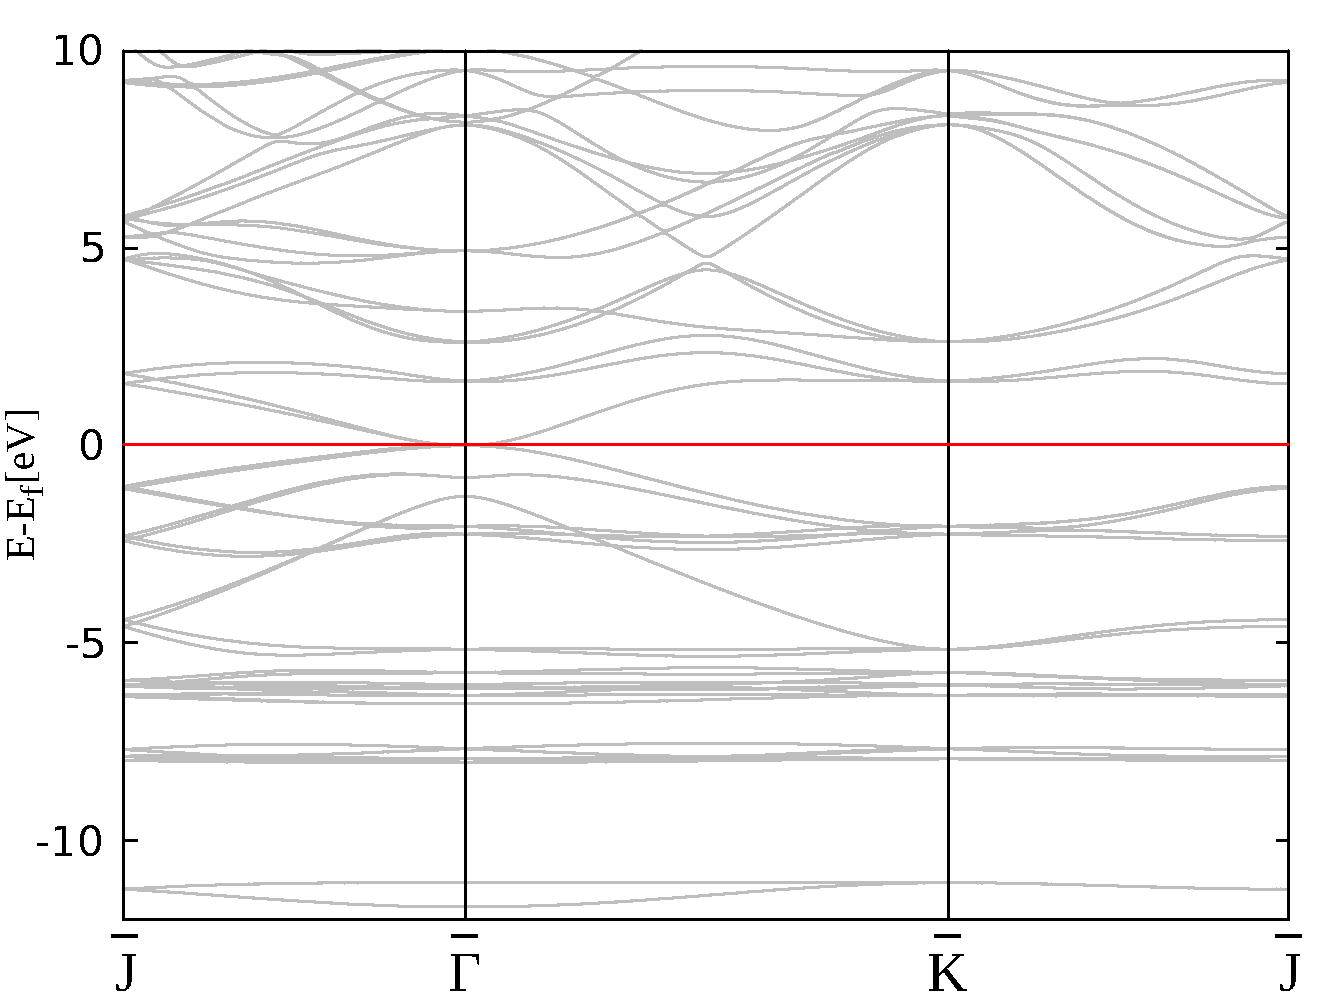
\includegraphics[width=\linewidth]{andere_bilder/0_bulk_-12_10.pdf}
			\caption{PBBS for $k_z$ is equal to zero.}
			\vspace{14pt}
		\end{subfigure}
		\hfill
%		\begin{subfigure}[c]{.48\linewidth}
%			\centering
%			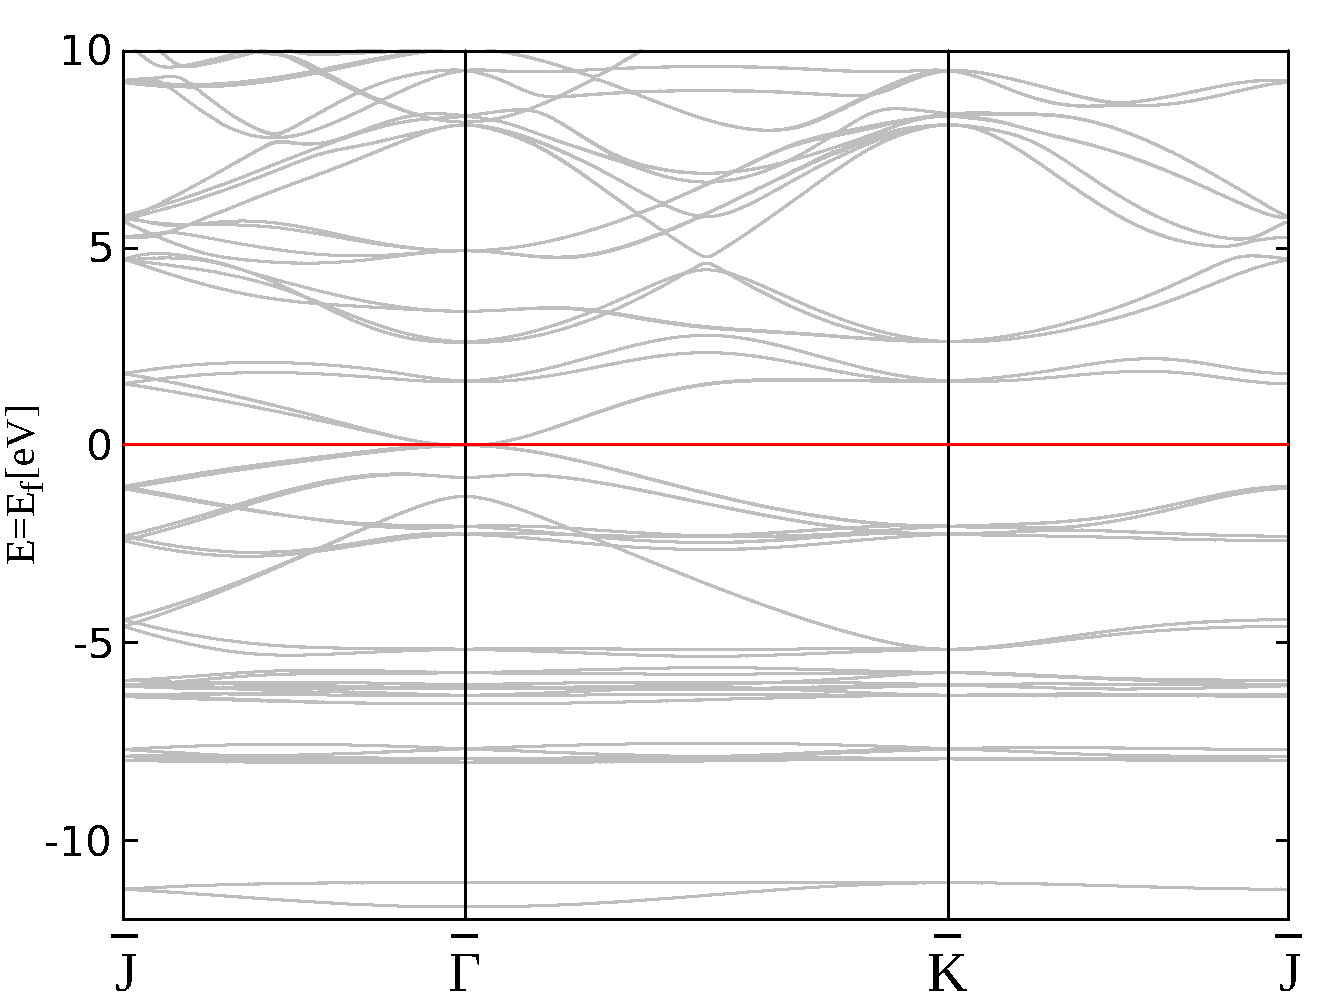
\includegraphics[width=\linewidth]{2_bulk_-12_10.pdf}
%			\caption{PBBS calculations with $k_z = 0$, $1/40\cdot k_{z,\text{max}}$, $1/20\cdot k_{z,\text{max}}$}
%		\end{subfigure}
		\begin{subfigure}[c]{.48\linewidth}
			\centering
			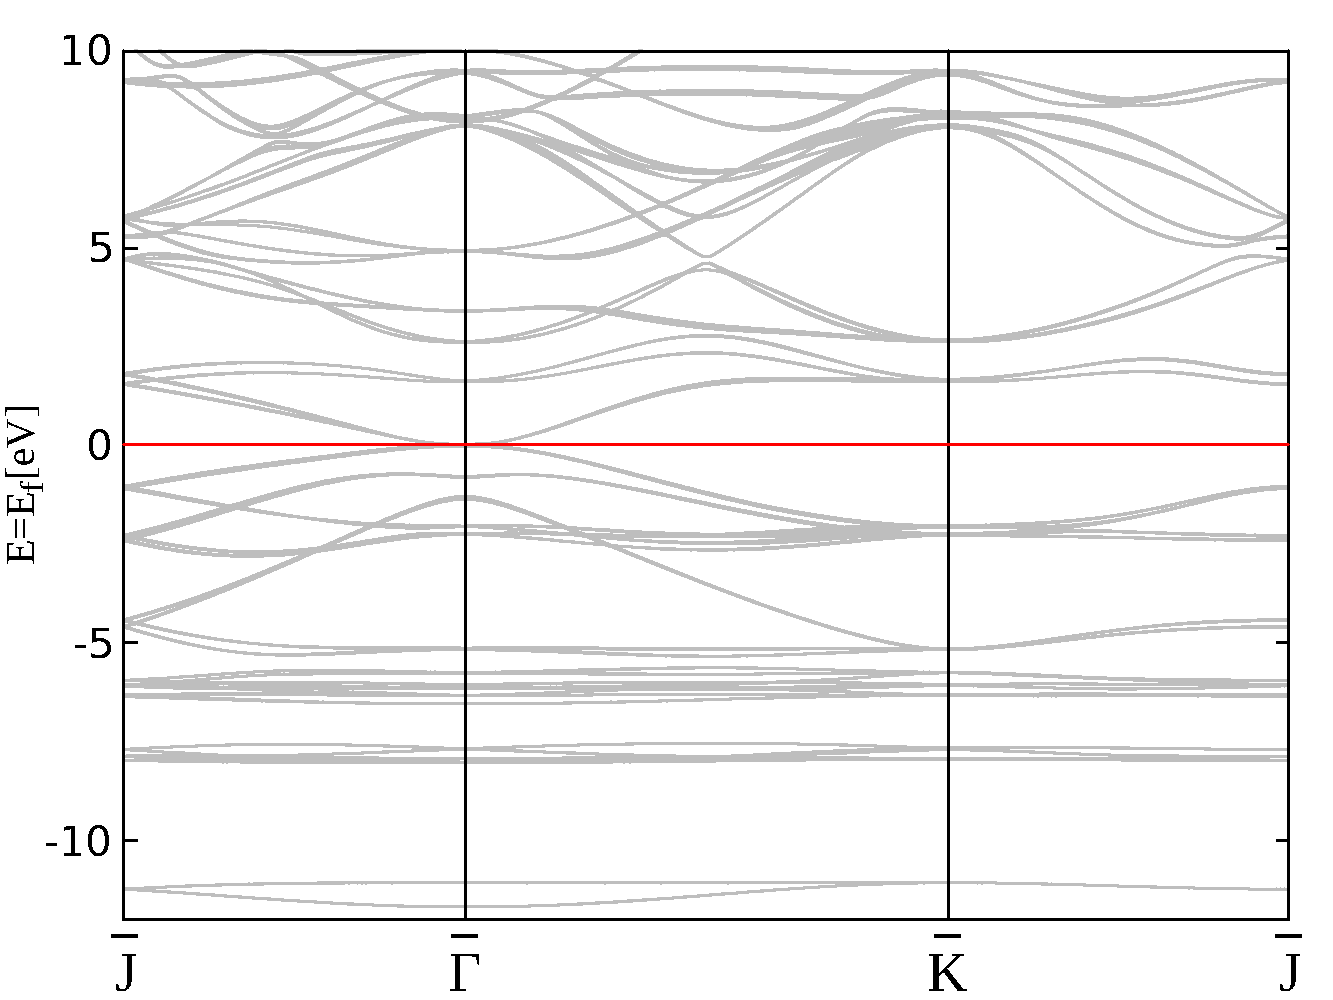
\includegraphics[width=\linewidth]{andere_bilder/4_bulk_-12_10.pdf}
			\caption{Ensemble for PBBS for $k_z$ having values from 0 to $1/10\cdot k_{z,\text{max}}$}
		\end{subfigure}
%		\hfill
%		\begin{subfigure}[c]{.48\linewidth}
%			\centering
%			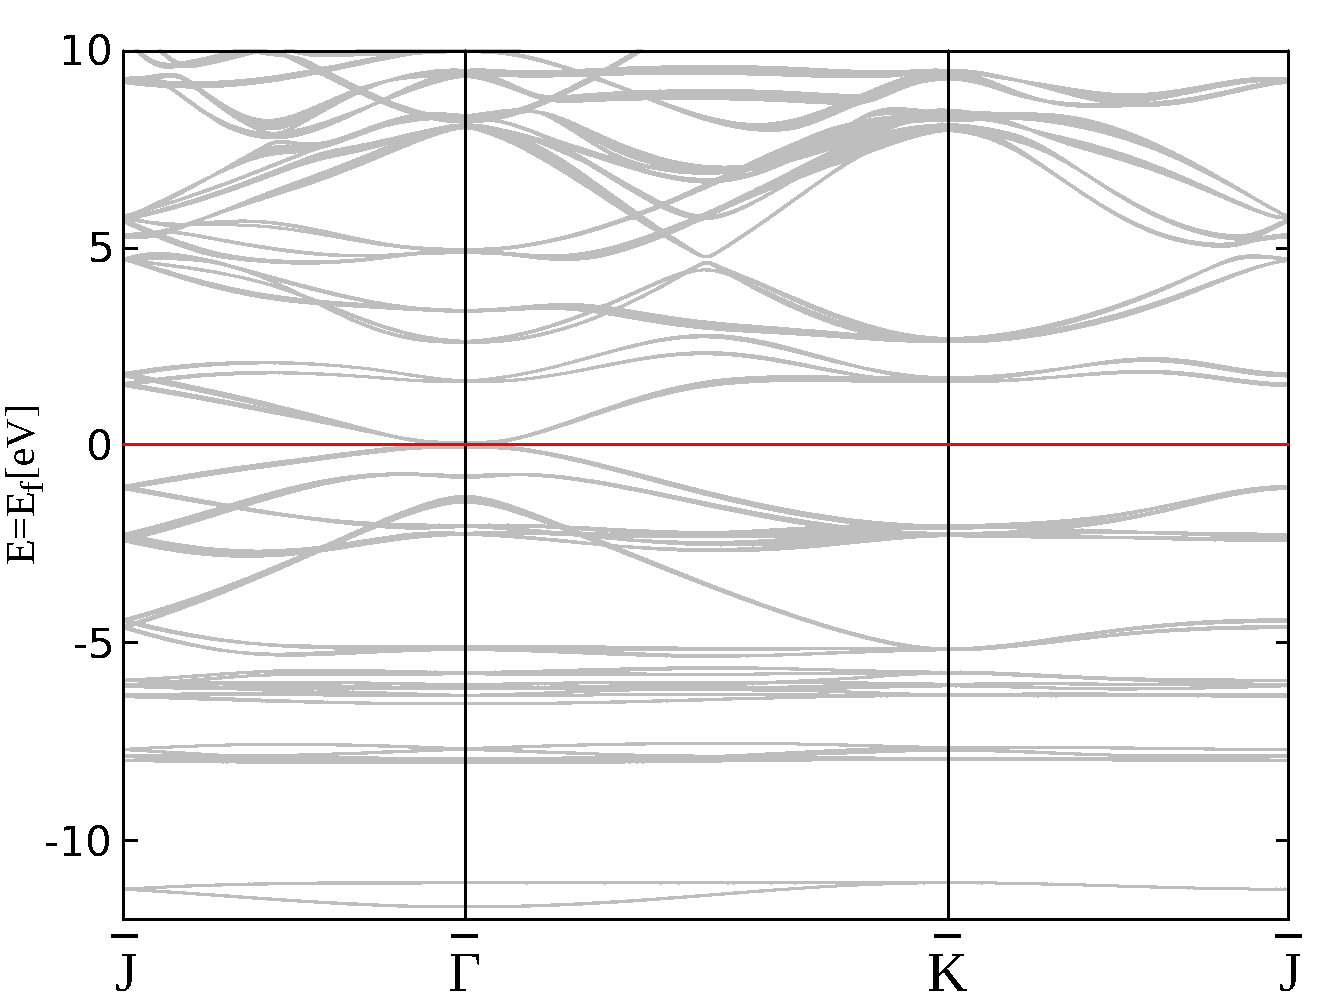
\includegraphics[width=\linewidth]{6_bulk_-12_10.pdf}
%			\caption{PBBS calculations with $k_z$ from 0 to $6/40\cdot k_{z,\text{max}}$}
%		\end{subfigure}
		\begin{subfigure}[c]{.48\linewidth}
			\centering
			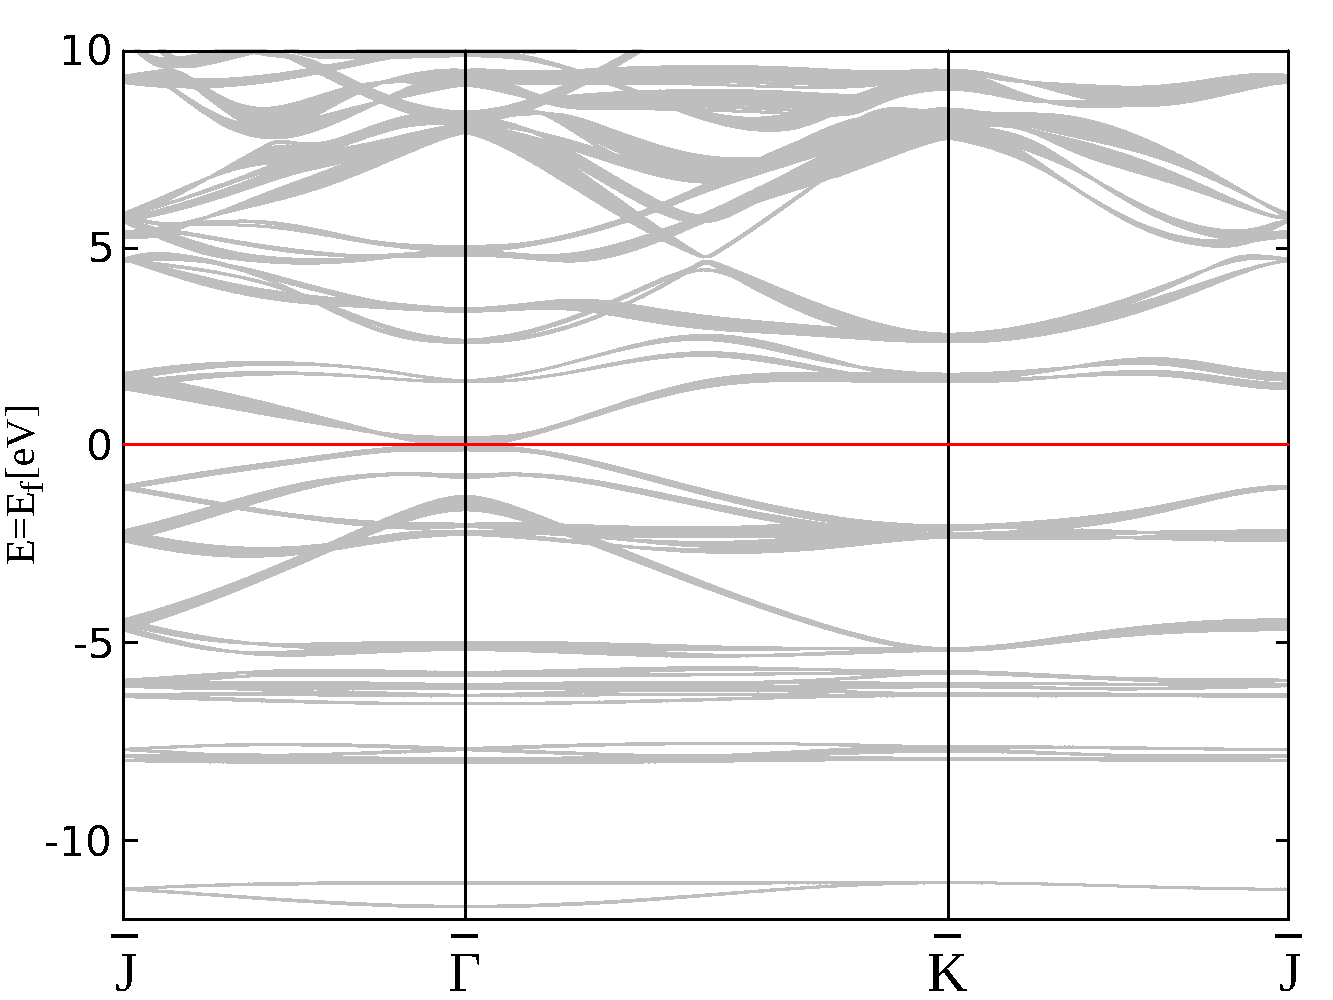
\includegraphics[width=\linewidth]{andere_bilder/10_bulk_-12_10.pdf}
			\caption{Ensemble for PBBS for $k_z$ having values from 0 to $1/4\cdot k_{z,\text{max}}$} 
		\end{subfigure}
		\hfill
		\begin{subfigure}[c]{.48\linewidth}
			\centering 
			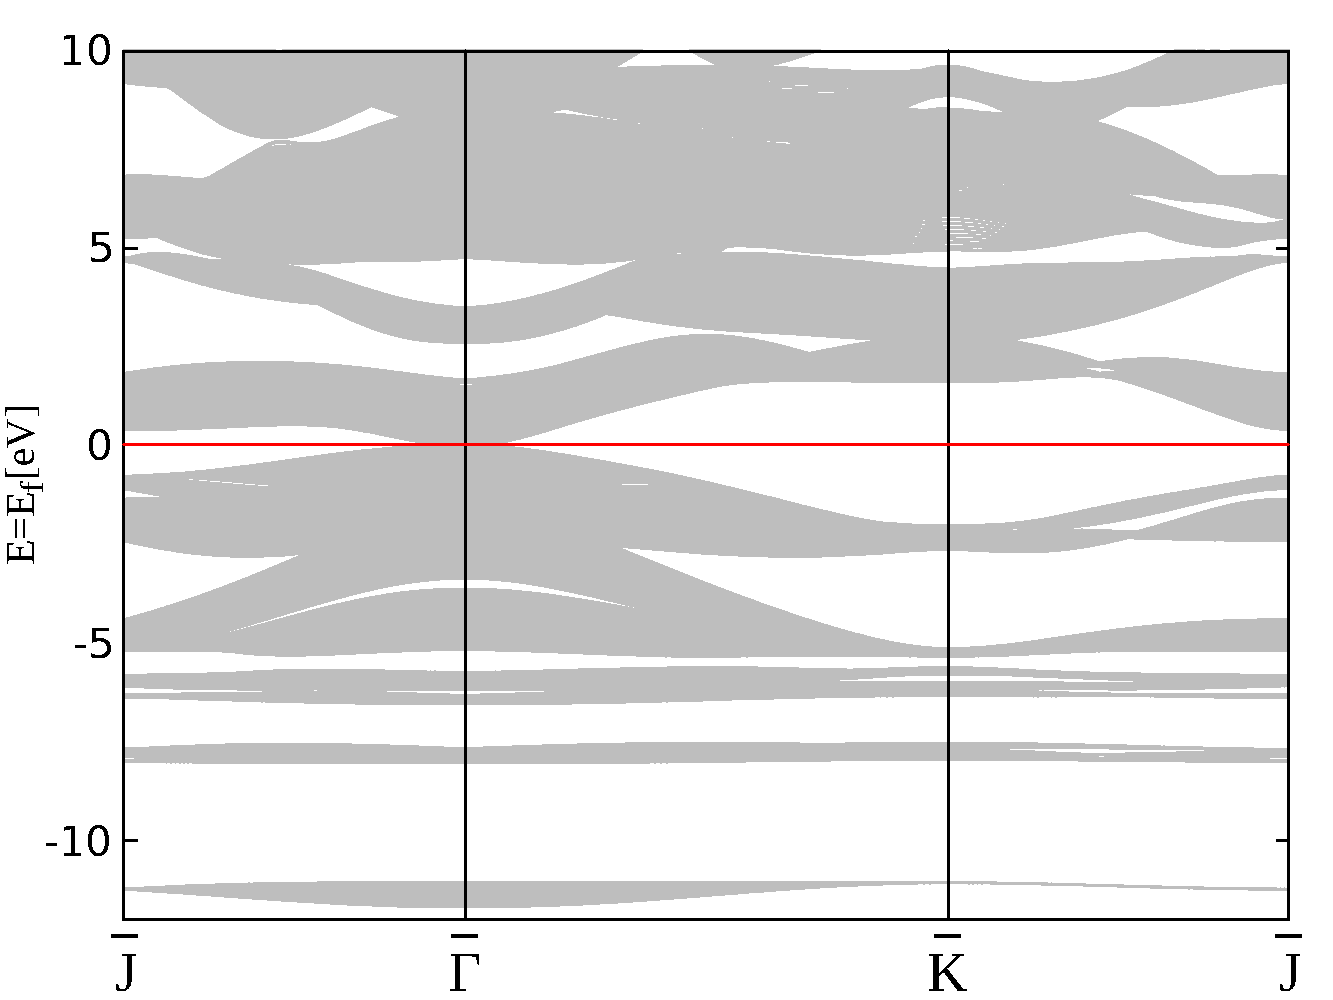
\includegraphics[width=\linewidth]{andere_bilder/bulk_-12_10.pdf}
			\caption{Whole PBBS for all the values of $k_z$ going from 0 to $k_{z,\text{max}}$} \label{bulk_PBBS}
		\end{subfigure}
		\caption{Generation of projected bulk band structure of HgTe} \label{bulk_band_structure_generation}
	\end{figure}

%Te-Hg termination	
	\begin{figure}[htbp]
		\begin{subfigure}[c]{.48\linewidth}
			\centering
			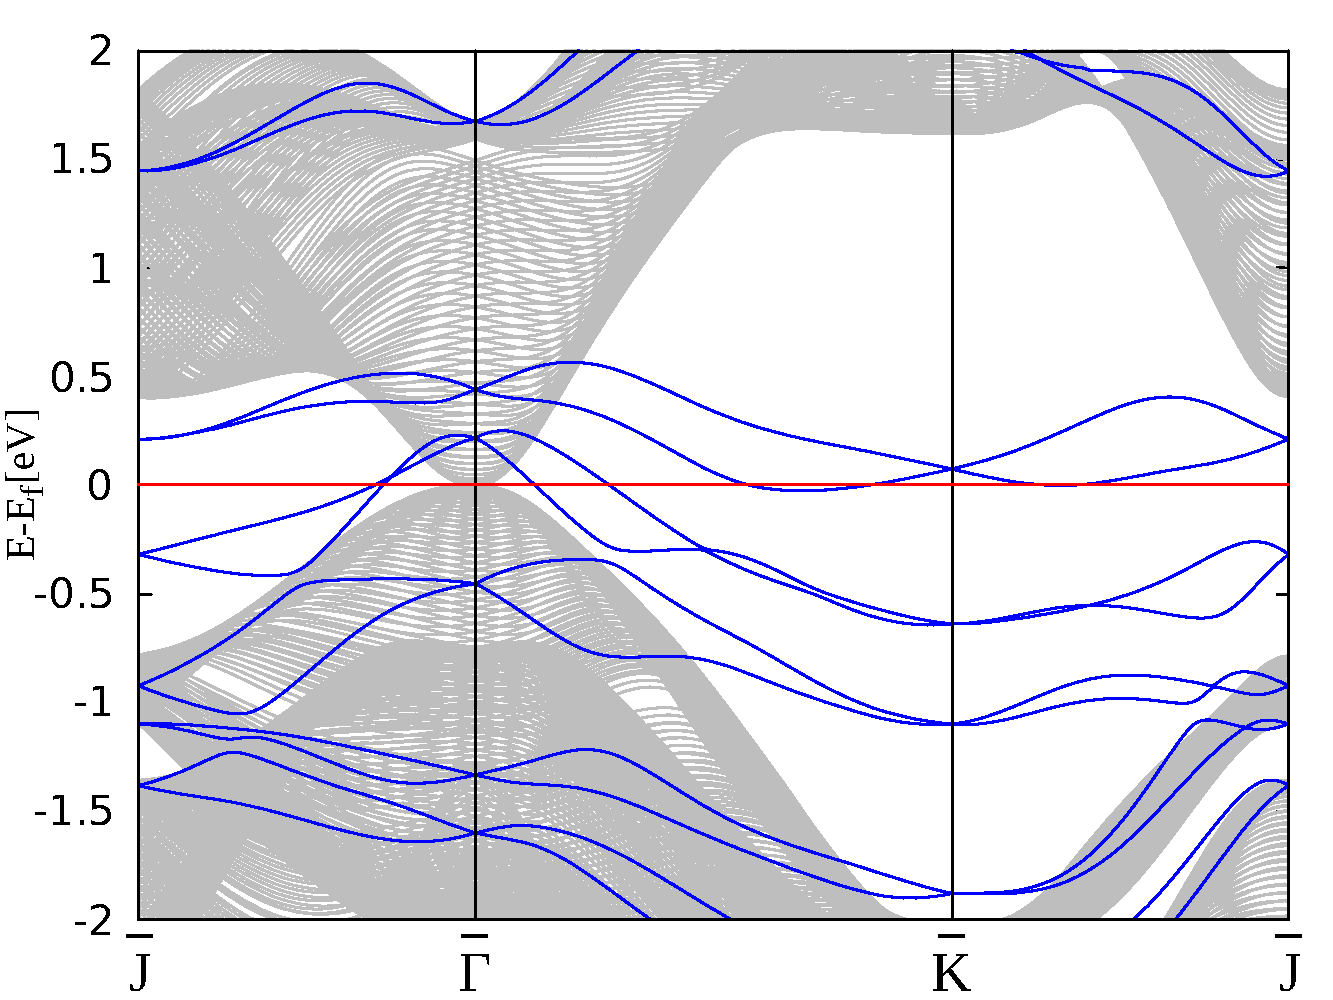
\includegraphics[width=\linewidth]{Te_and_Hg_termination/no_H_bulk+4_layers_no_dos_-2_2.pdf}
			\caption{4 layers without hydrogens passivating the Te termination}
		\end{subfigure}
		\hfill
		\begin{subfigure}[c]{.48\linewidth}
			\centering
			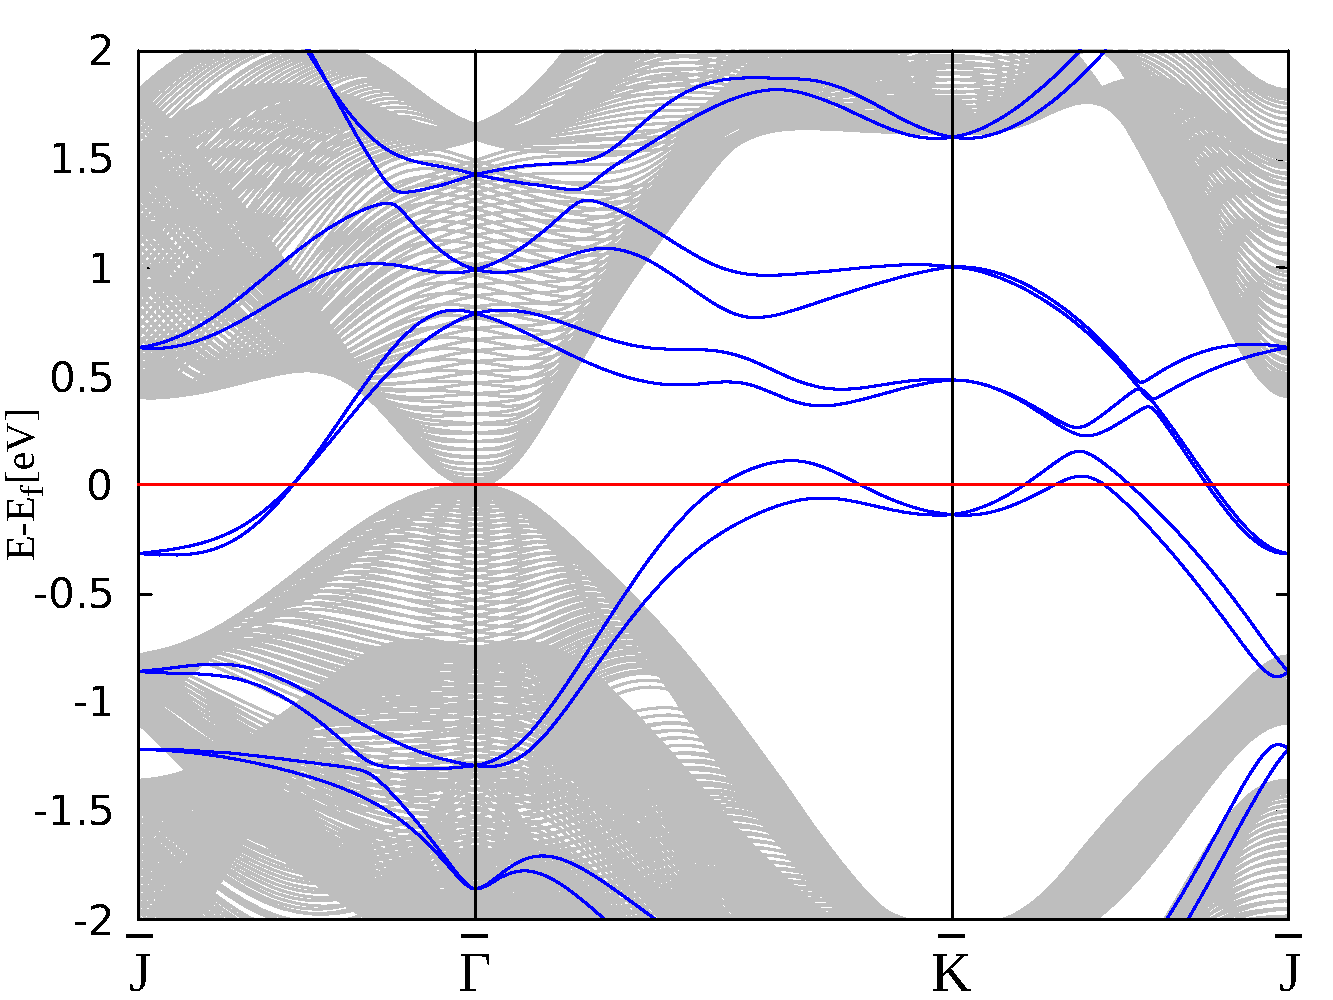
\includegraphics[width=\linewidth]{Te_and_Hg_termination/bulk+4_layers_no_dos_-2_2.pdf}
			\caption{4 layers with hydrogens on the bottom passivating the Te surface terminations}
		\end{subfigure}
		\begin{subfigure}[c]{.48\linewidth}
			\centering
			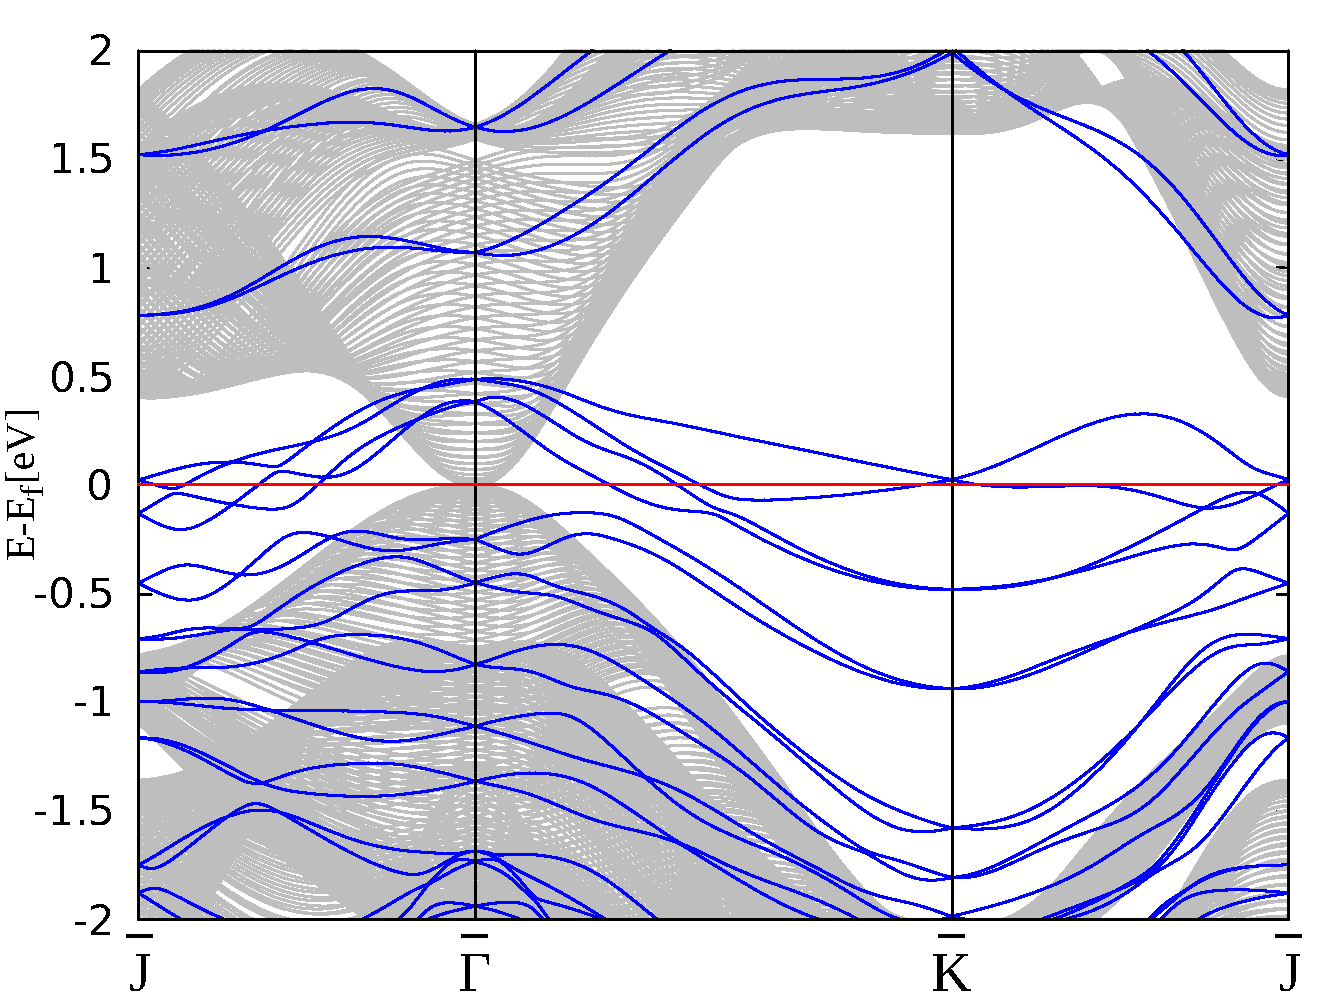
\includegraphics[width=\linewidth]{Te_and_Hg_termination/no_H_bulk+8_layers_no_dos_-2_2.pdf}
			\caption{8 layers without hydrogens passivating the Te termination}
		\end{subfigure}
		\hfill
		\begin{subfigure}[c]{.48\linewidth}
			\centering
			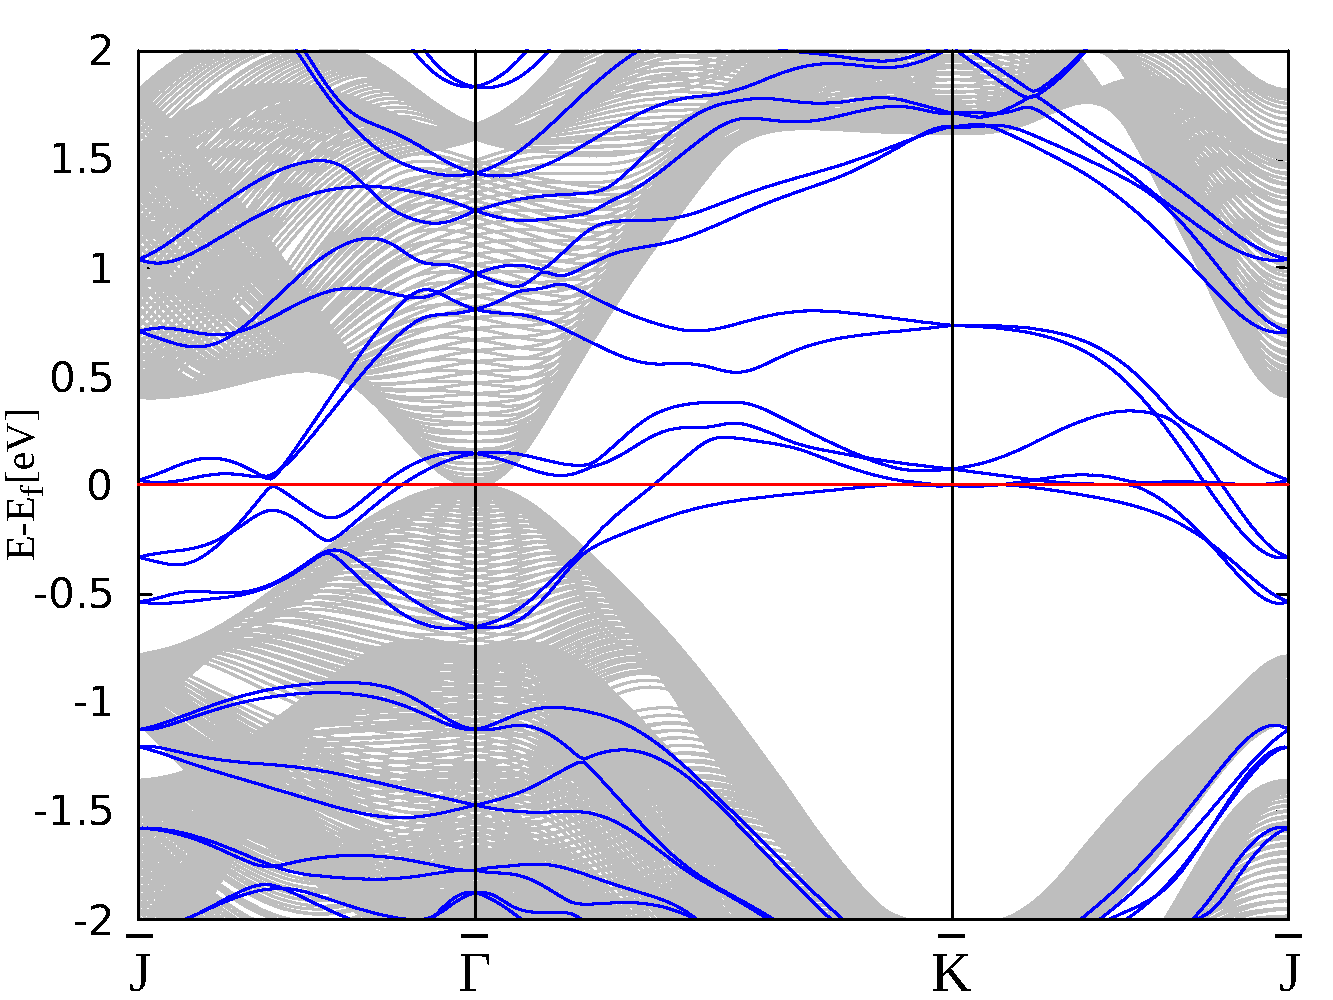
\includegraphics[width=\linewidth]{Te_and_Hg_termination/bulk+8_layers_no_dos_-2_2.pdf}
			\caption{8 layers with hydrogens on the bottom passivating the Te surface terminations}
		\end{subfigure}
		\begin{subfigure}[c]{.48\linewidth}
			\centering 
			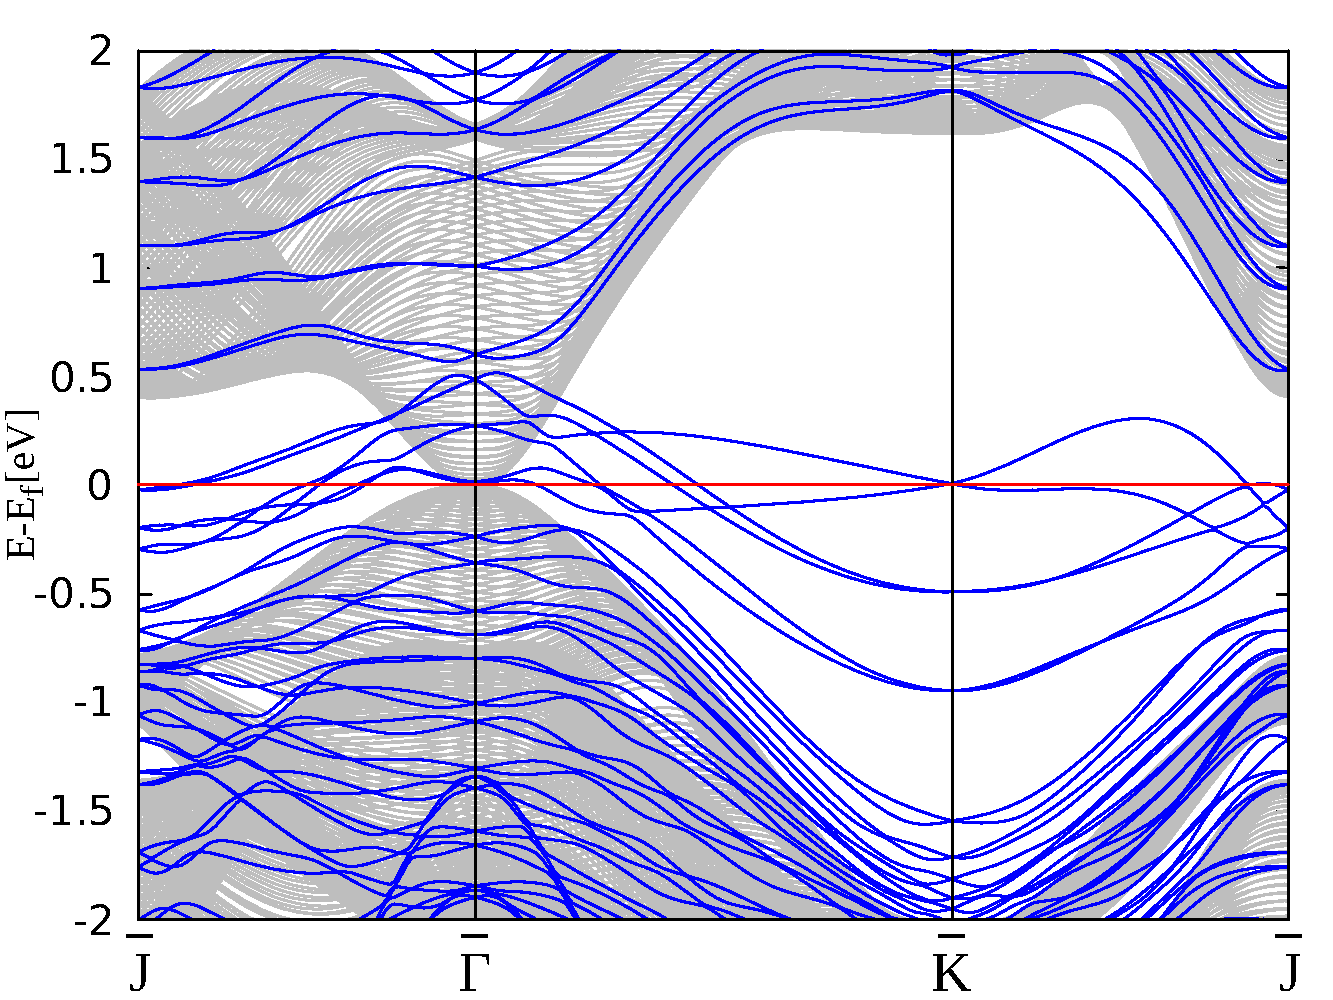
\includegraphics[width=\linewidth]{Te_and_Hg_termination/no_H_bulk+16_layers_no_dos_-2_2.pdf}
			\caption{16 layers without hydrogens passivating the Te termination} \label{}
		\end{subfigure}
		\hfill
		\begin{subfigure}[c]{.48\linewidth}
			\centering
			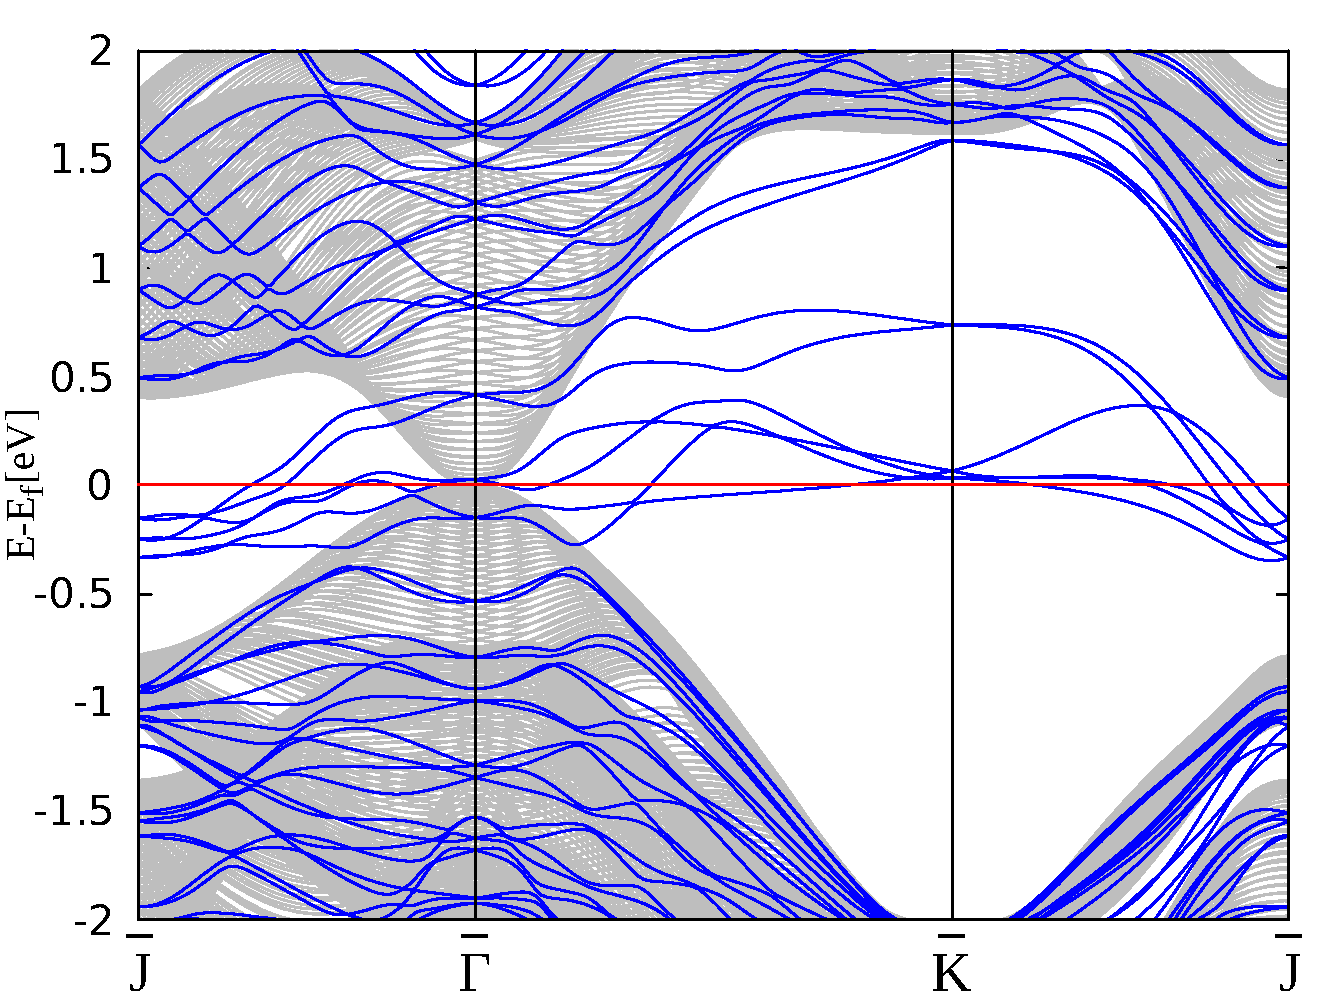
\includegraphics[width=\linewidth]{Te_and_Hg_termination/bulk+16_layers_no_dos_-2_2.pdf}
			\caption{16 layers with hydrogens on the bottom passivating the Te surface terminations}
		\end{subfigure}
		\caption{PBBS and surface band structure for Te-Hg terminations} 
		\label{bulk+surface_even_layers}
	\end{figure}

%Te termination	
	\begin{figure}[htbp]
		\begin{subfigure}[c]{.48\linewidth}
			\centering
			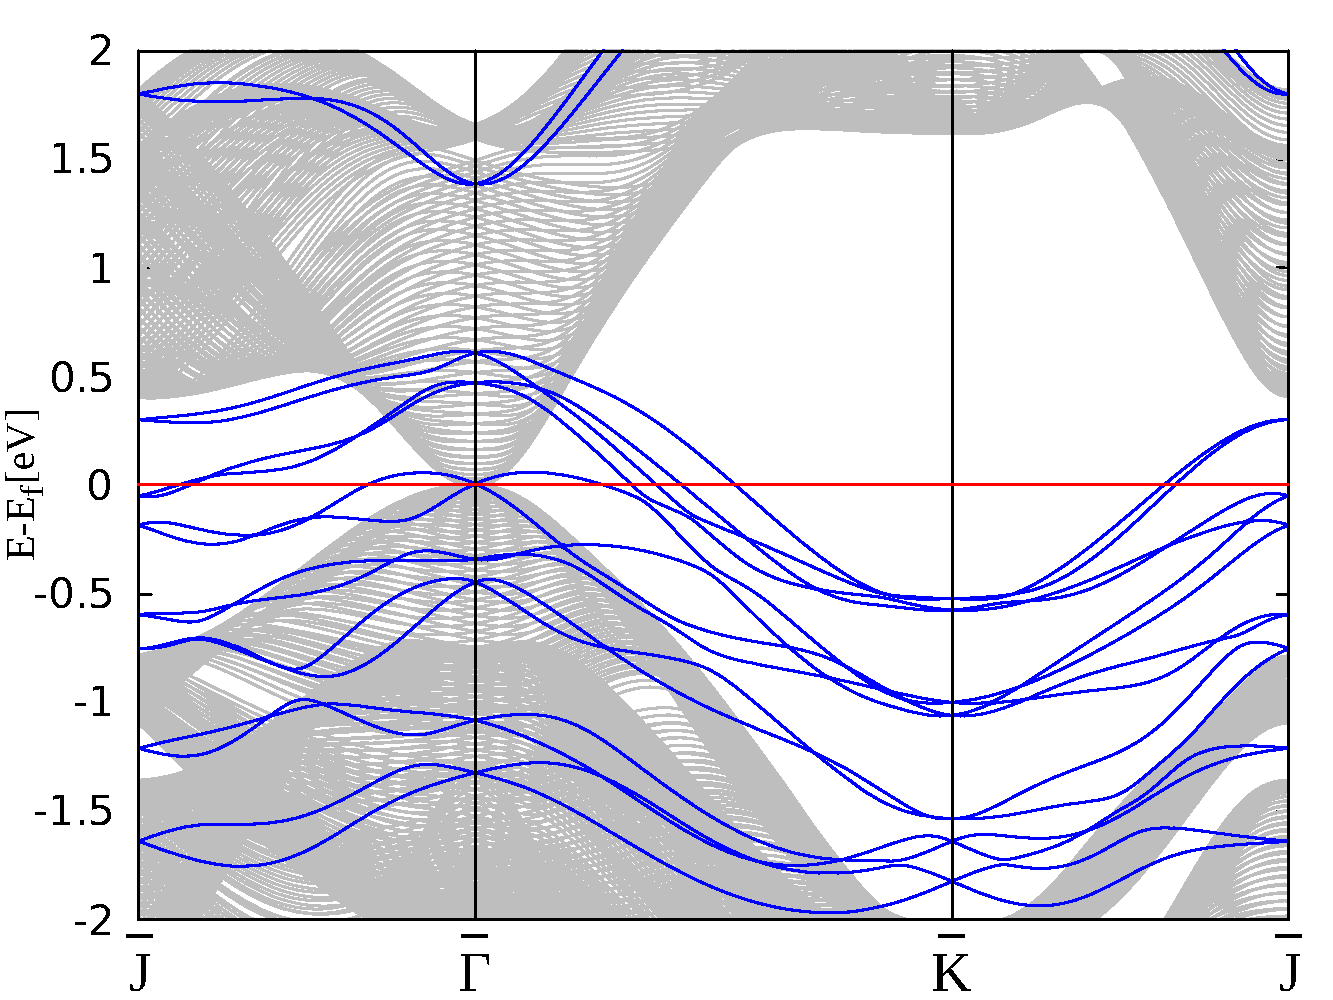
\includegraphics[width=\linewidth]{Te_termination/no_H_bulk+5_layers_no_dos_-2_2.pdf}
			\caption{5 layers without hydrogens passivating one of the surfaces}
		\end{subfigure}
		\hfill
		\begin{subfigure}[c]{.48\linewidth}
			\centering
			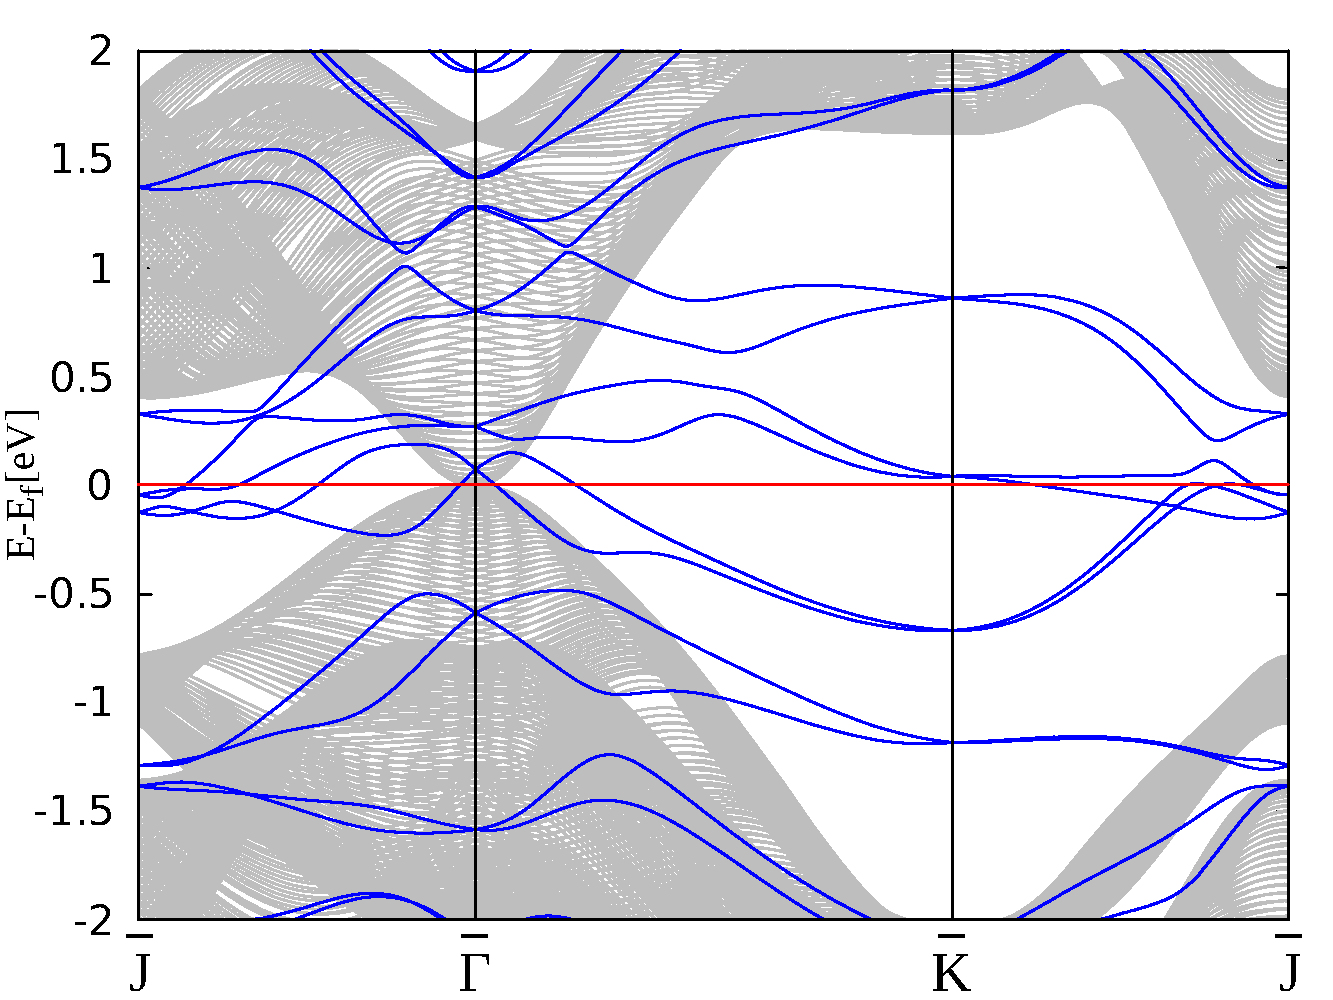
\includegraphics[width=\linewidth]{Te_termination/bulk+5_layers_no_dos_-2_2.pdf}
			\caption{5 layers with hydrogens on the bottom passivating one of the Te surface terminations}
		\end{subfigure}
		\begin{subfigure}[c]{.48\linewidth}
			\centering
			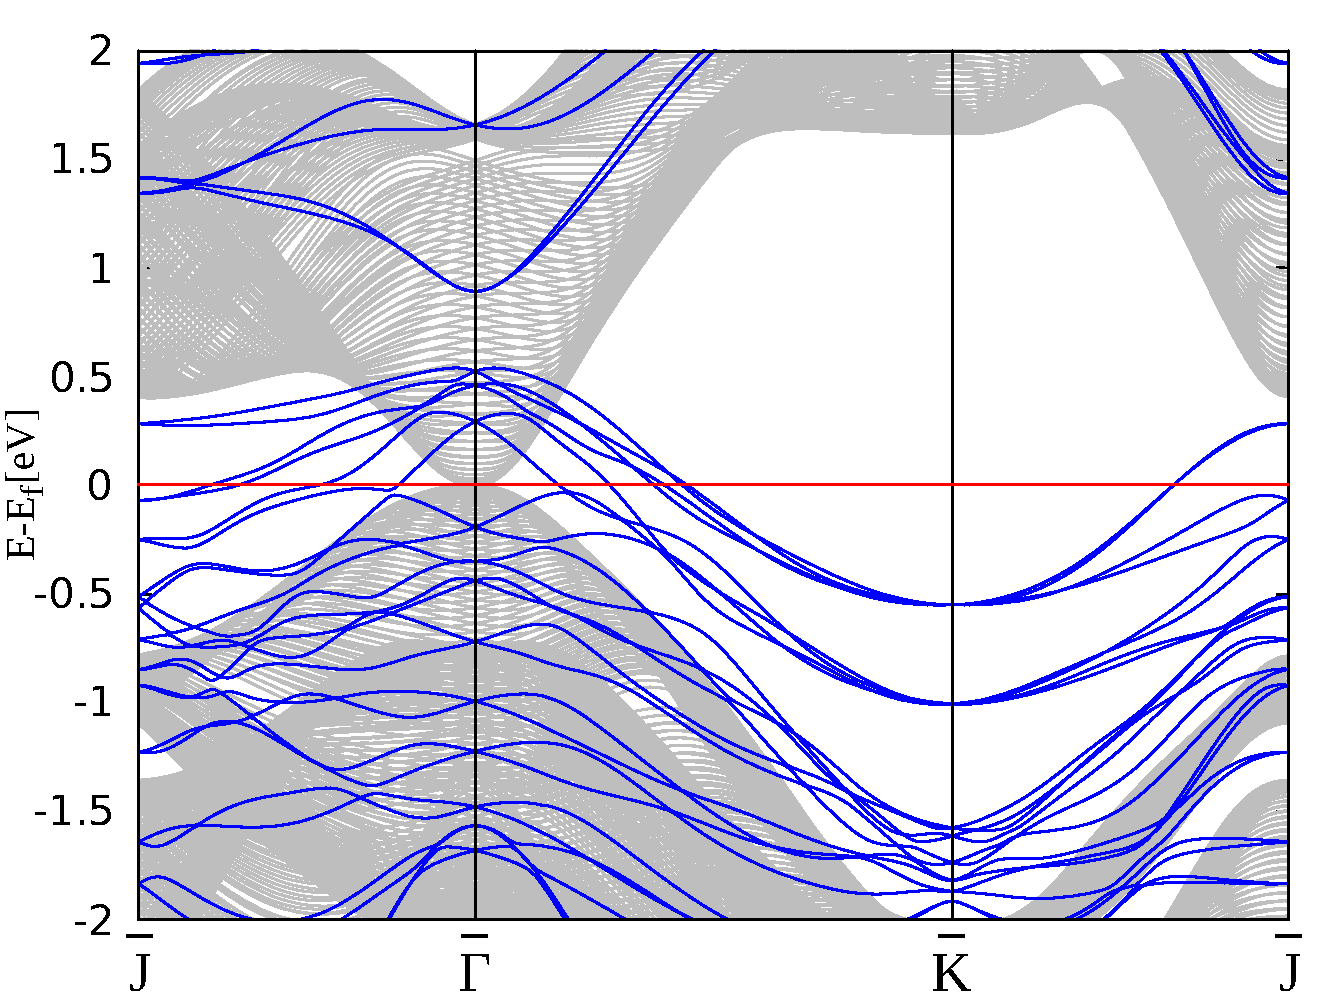
\includegraphics[width=\linewidth]{Te_termination/no_H_bulk+9_layers_no_dos_-2_2.pdf}
			\caption{9 layers without hydrogens passivating one of the surfaces}
		\end{subfigure}
		\hfill
		\begin{subfigure}[c]{.48\linewidth}
			\centering
			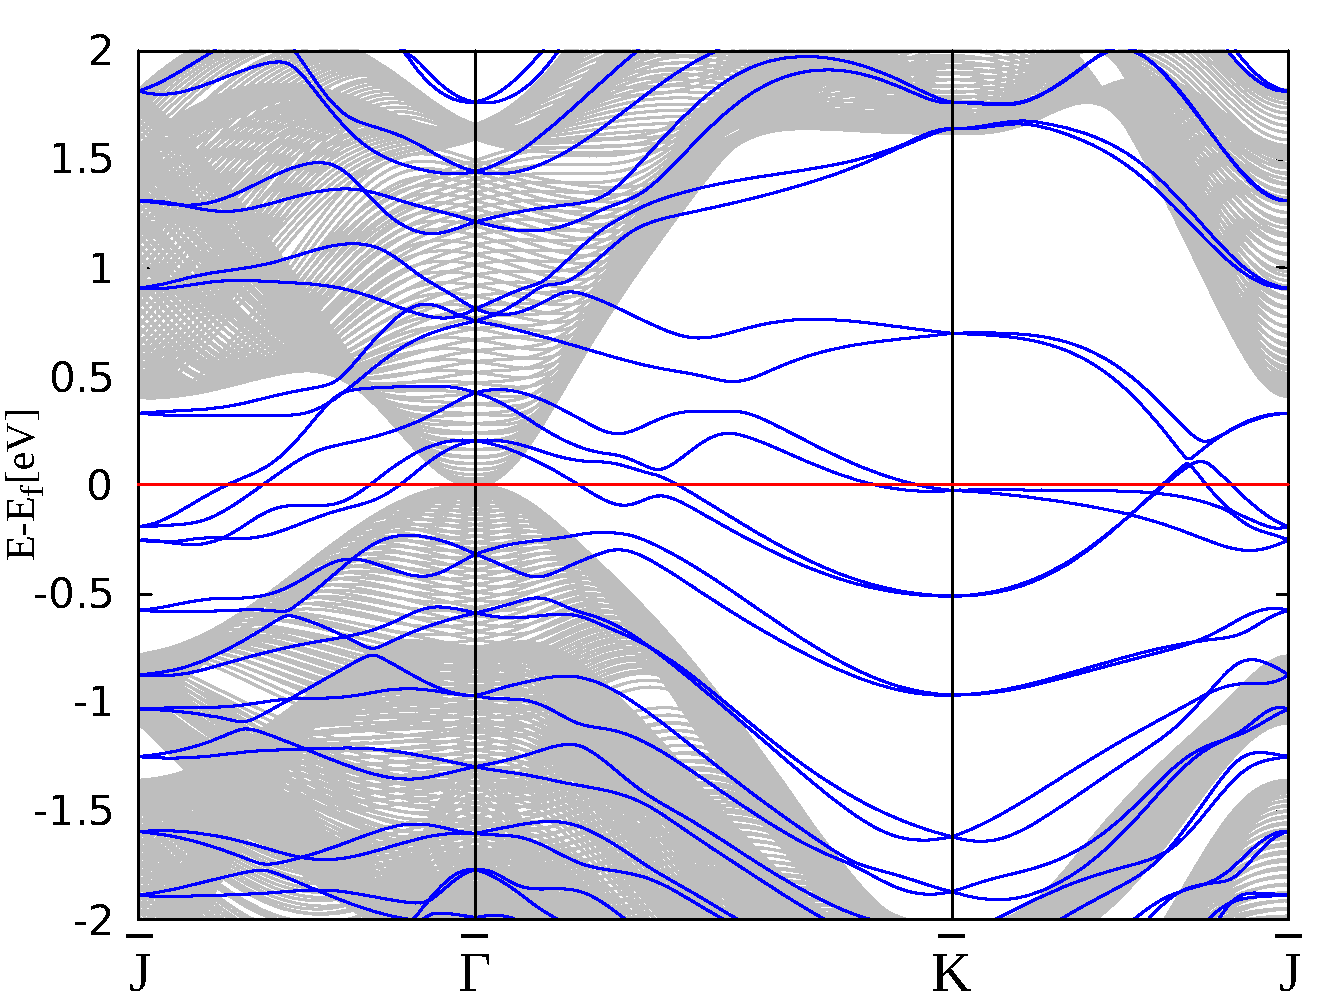
\includegraphics[width=\linewidth]{Te_termination/bulk+9_layers_no_dos_-2_2.pdf}
			\caption{9 layers with hydrogens on the bottom passivating one of the Te surface terminations}
		\end{subfigure}
		\begin{subfigure}[c]{.48\linewidth}
			\centering 
			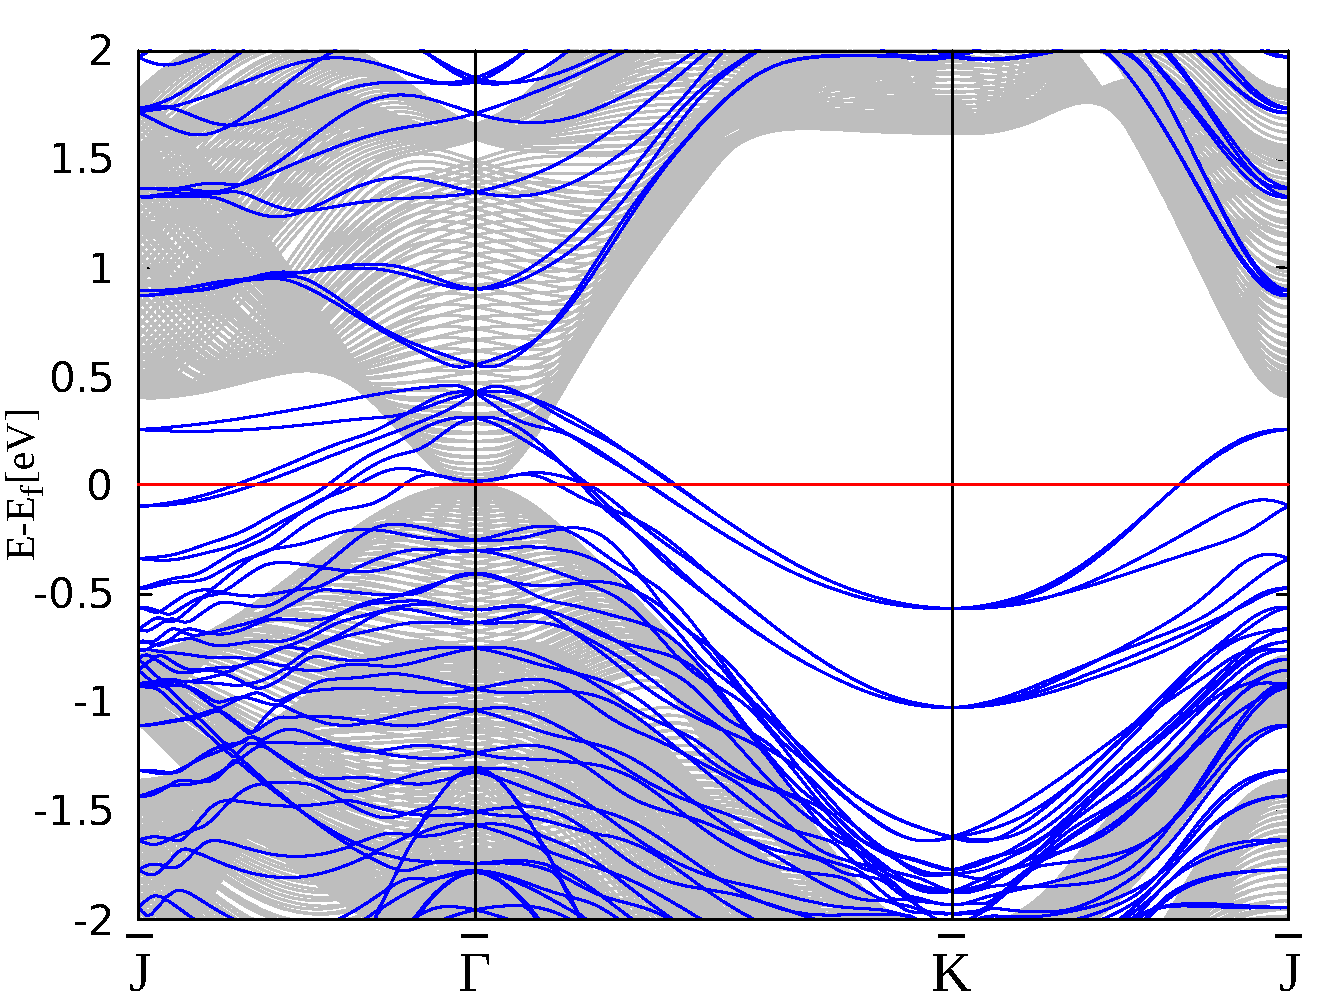
\includegraphics[width=\linewidth]{Te_termination/no_H_bulk+17_layers_no_dos_-2_2.pdf}
			\caption{17 layers without hydrogens passivating one of the surfaces} 
		\end{subfigure}
		\hfill
		\begin{subfigure}[c]{.48\linewidth}
			\centering
			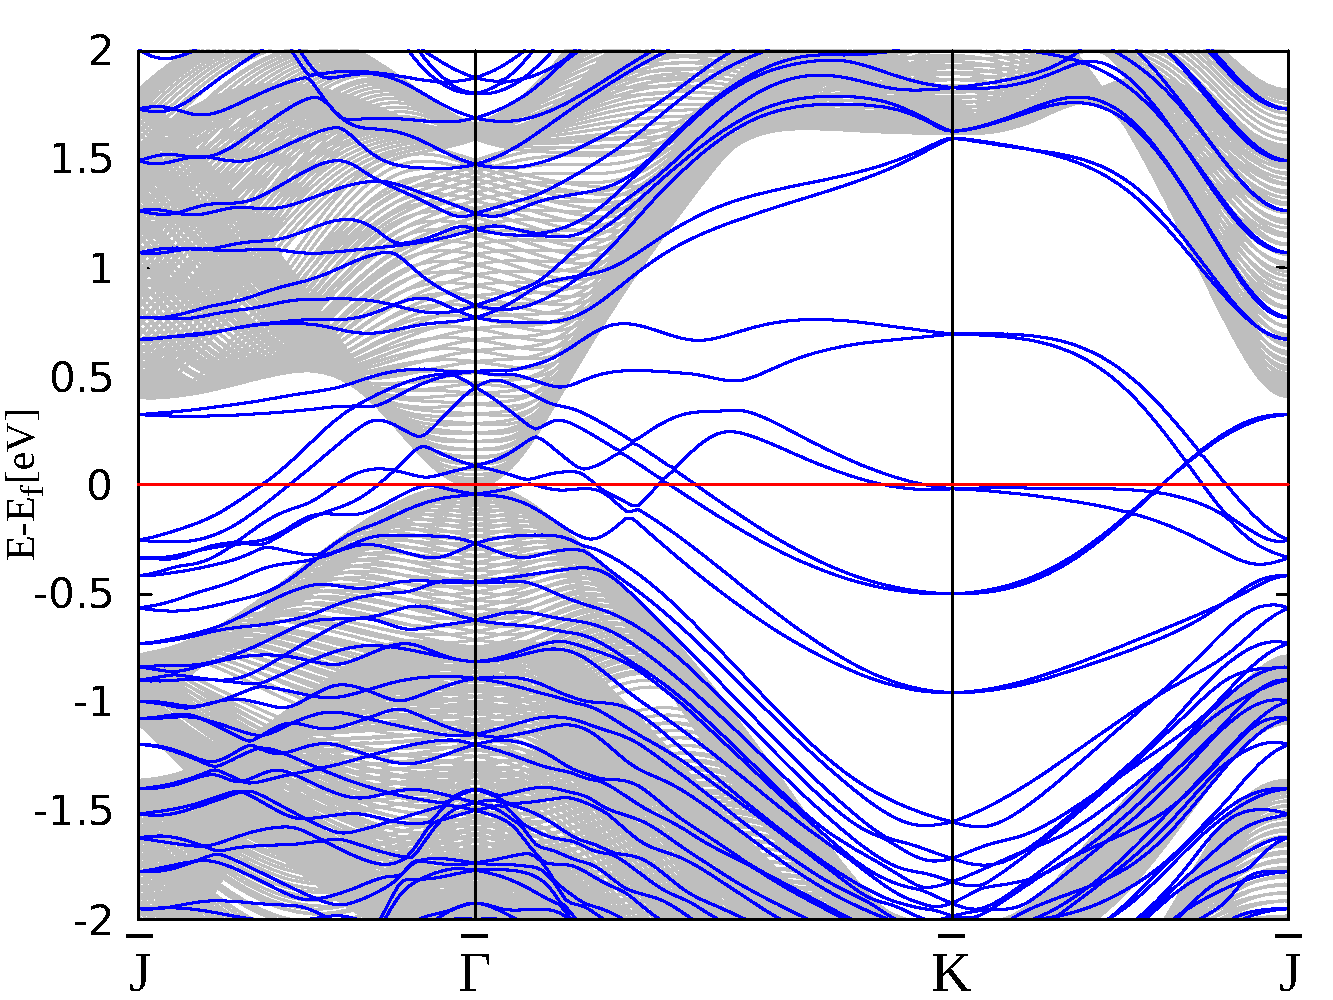
\includegraphics[width=\linewidth]{Te_termination/bulk+17_layers_no_dos_-2_2.pdf}
			\caption{17 layers with hydrogens on the bottom passivating one of the Te surface terminations}
		\end{subfigure}
		\caption{PBBS and surface band structure for symmetric Te termination on both surfaces of the slab} 
		\label{bulk+surface_odd_layers_Te}
	\end{figure}

%Hg termination	
	\begin{figure}[htbp]
		\begin{subfigure}[c]{.48\linewidth}
			\centering
			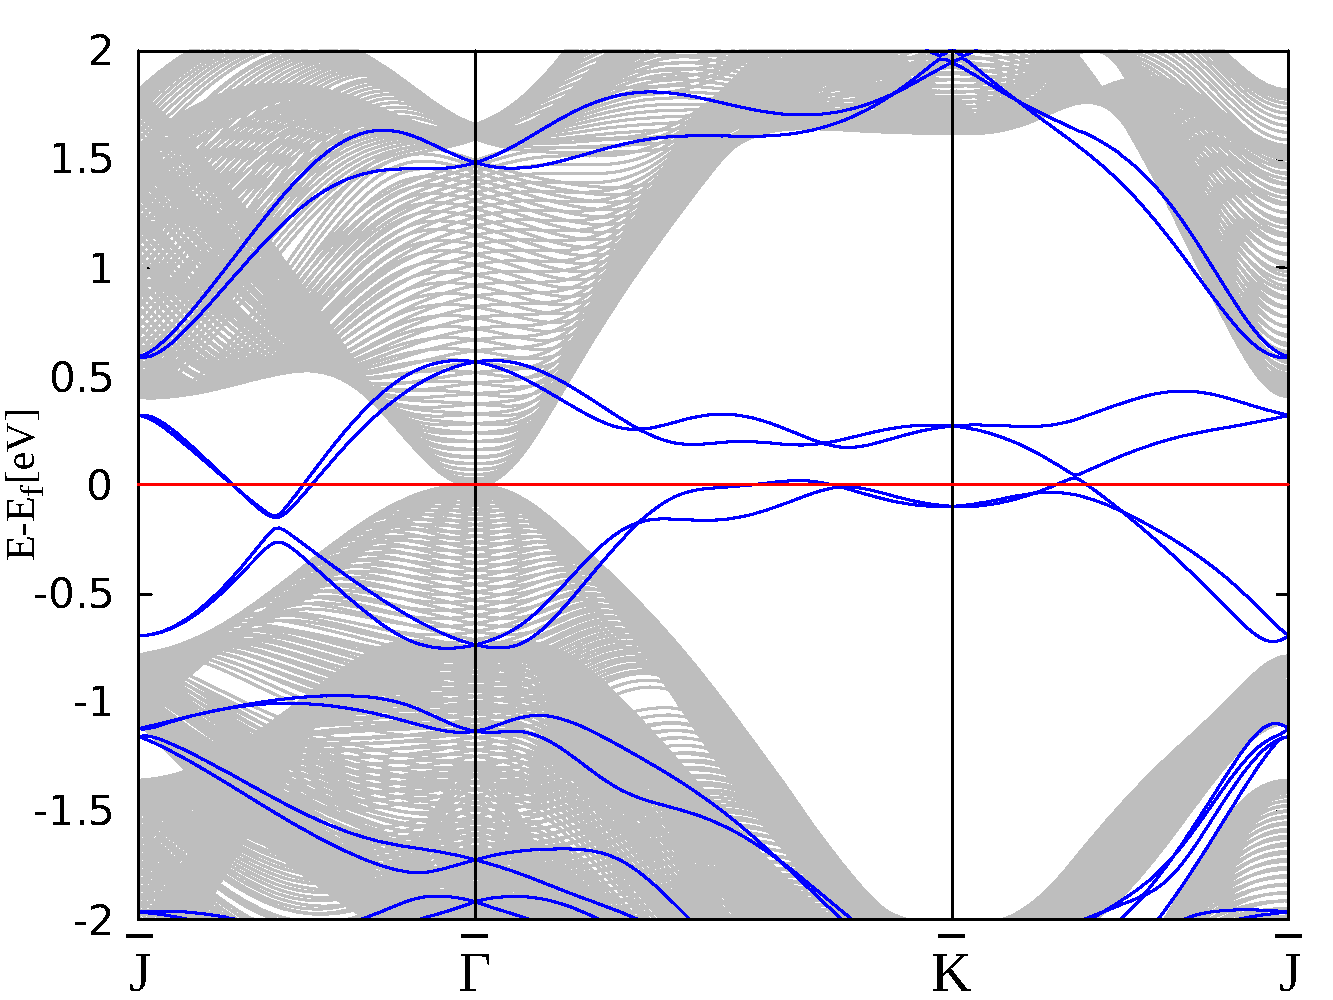
\includegraphics[width=\linewidth]{Hg_termination/no_H_bulk+5_layers_no_dos_-2_2.pdf}
			\caption{5 layers without hydrogens passivating one of the surfaces}
		\end{subfigure}
		\hfill
		\begin{subfigure}[c]{.48\linewidth}
			\centering
			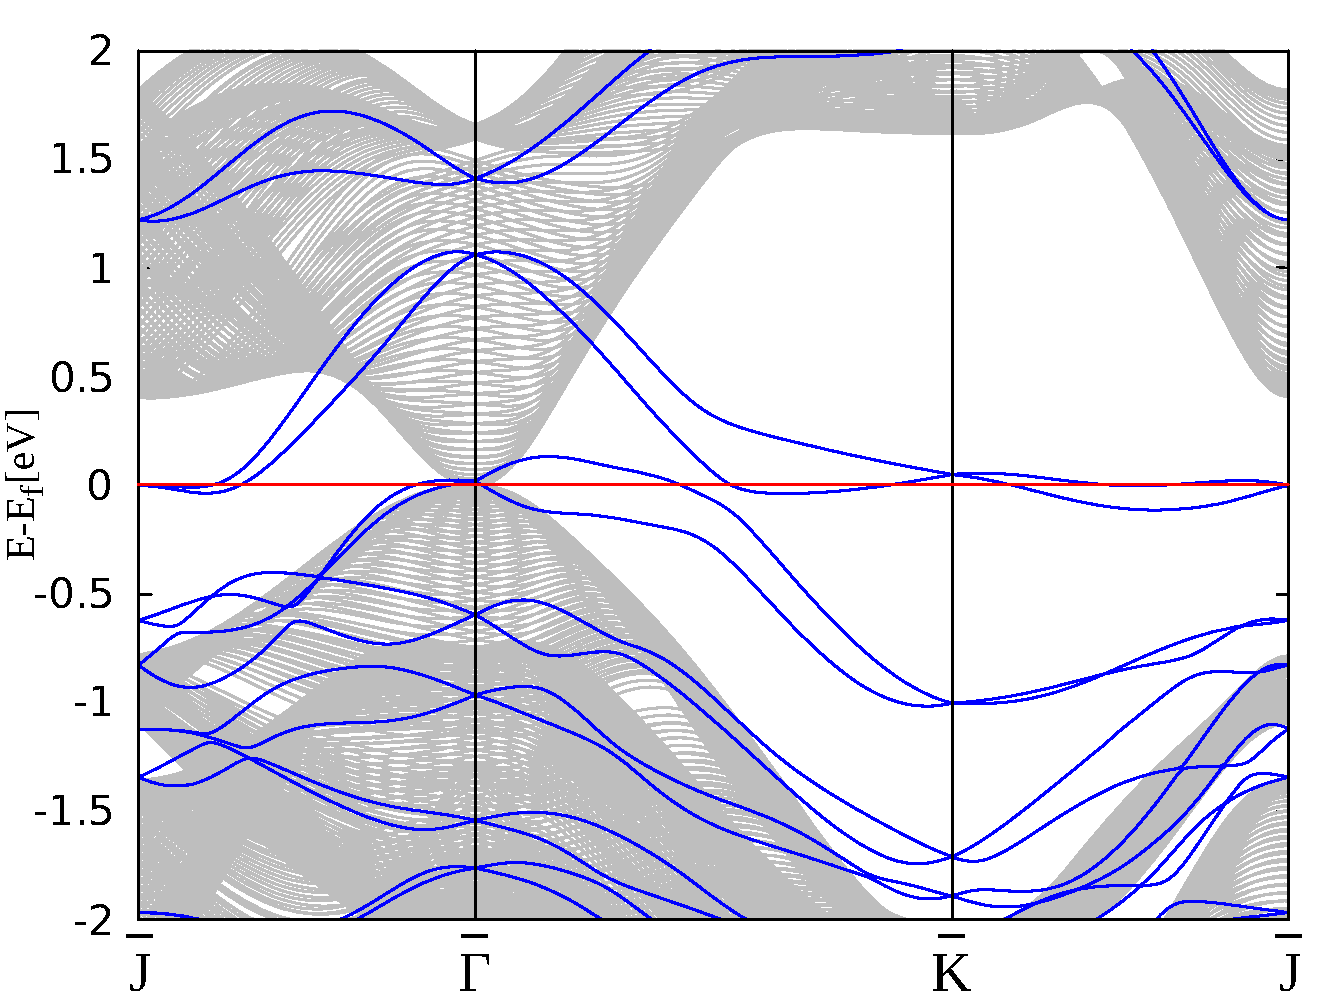
\includegraphics[width=\linewidth]{Hg_termination/bulk+5_layers_no_dos_-2_2.pdf}
			\caption{5 layers with hydrogens on the bottom passivating one of the Hg surface terminations}
		\end{subfigure}
		\begin{subfigure}[c]{.48\linewidth}
			\centering
			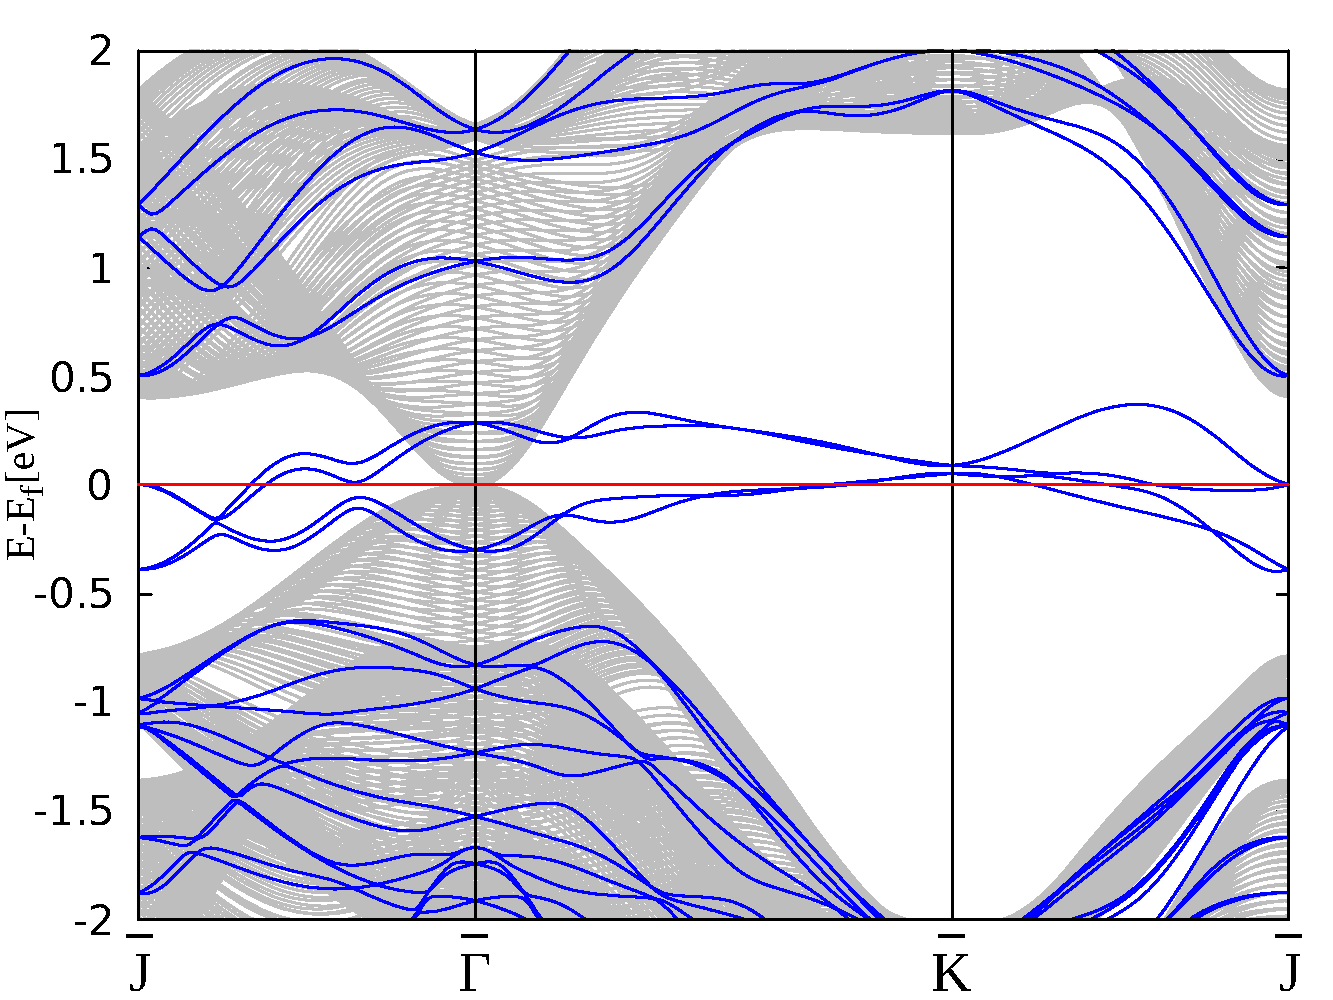
\includegraphics[width=\linewidth]{Hg_termination/no_H_bulk+9_layers_no_dos_-2_2.pdf}
			\caption{9 layers without hydrogens passivating one of the surfaces}
		\end{subfigure}
		\hfill
		\begin{subfigure}[c]{.48\linewidth}
			\centering
			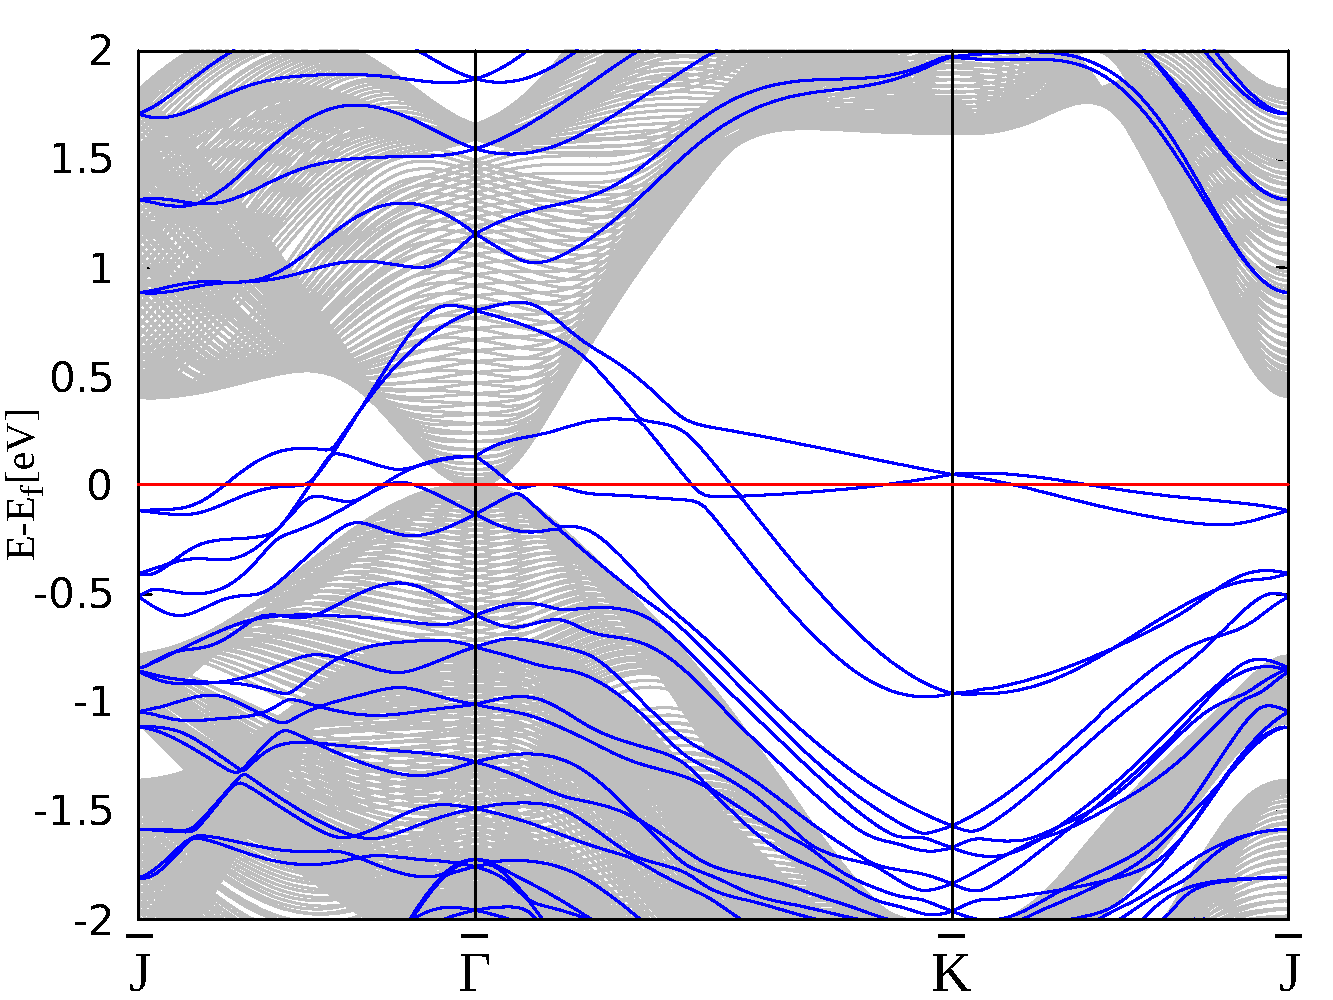
\includegraphics[width=\linewidth]{Hg_termination/bulk+9_layers_no_dos_-2_2.pdf}
			\caption{9 layers with hydrogens on the bottom passivating one of the Hg surface terminations}
		\end{subfigure}
		\begin{subfigure}[c]{.48\linewidth}
			\centering 
			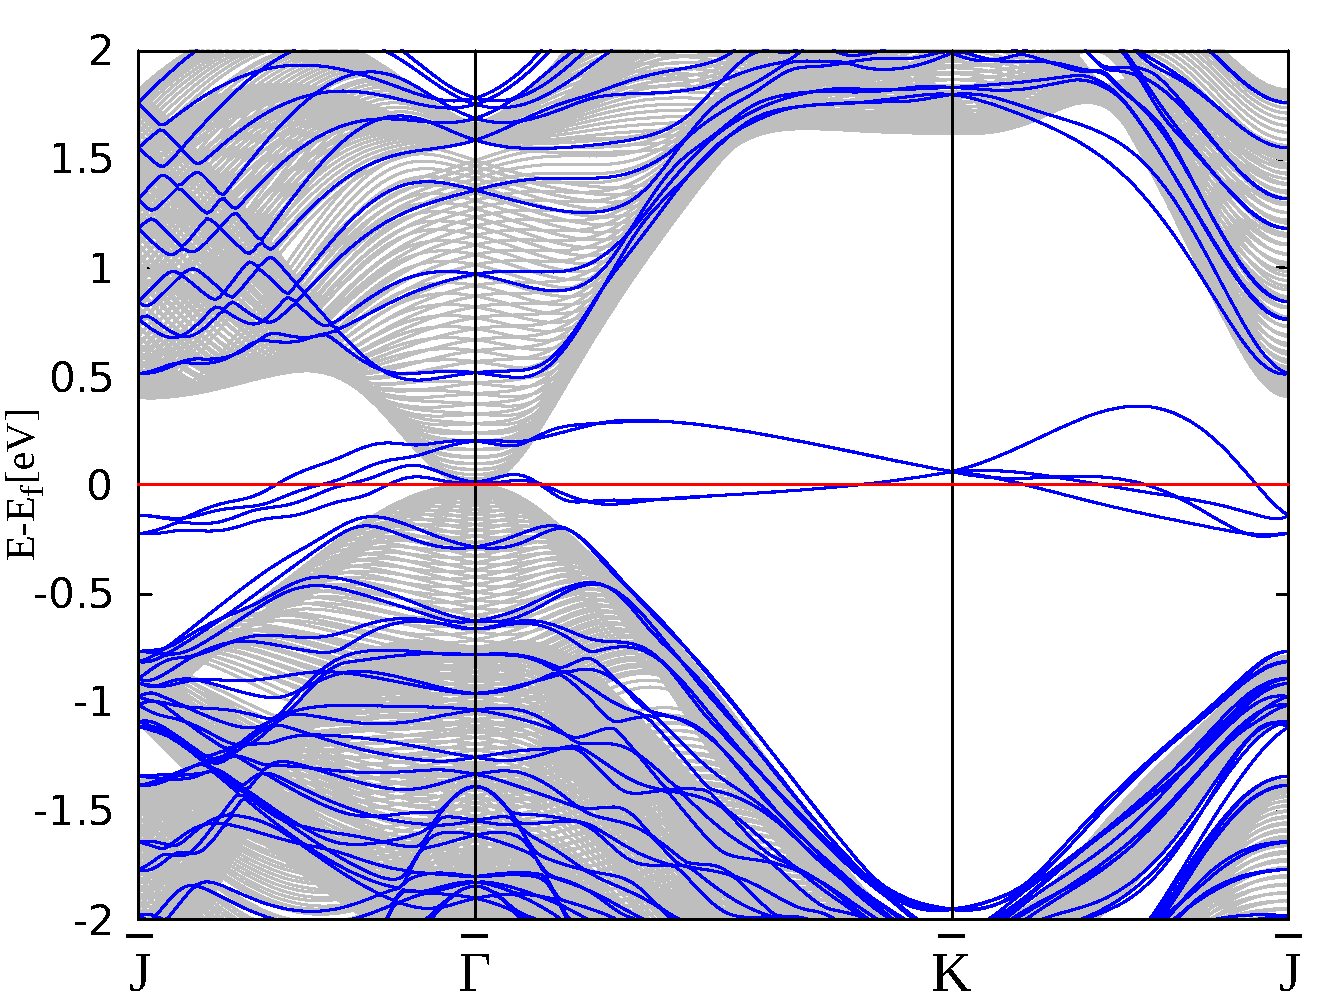
\includegraphics[width=\linewidth]{Hg_termination/no_H_bulk+17_layers_no_dos_-2_2.pdf}
			\caption{17 layers without hydrogens passivating one of the surfaces} \label{}
		\end{subfigure}
		\hfill
		\begin{subfigure}[c]{.48\linewidth}
			\centering
			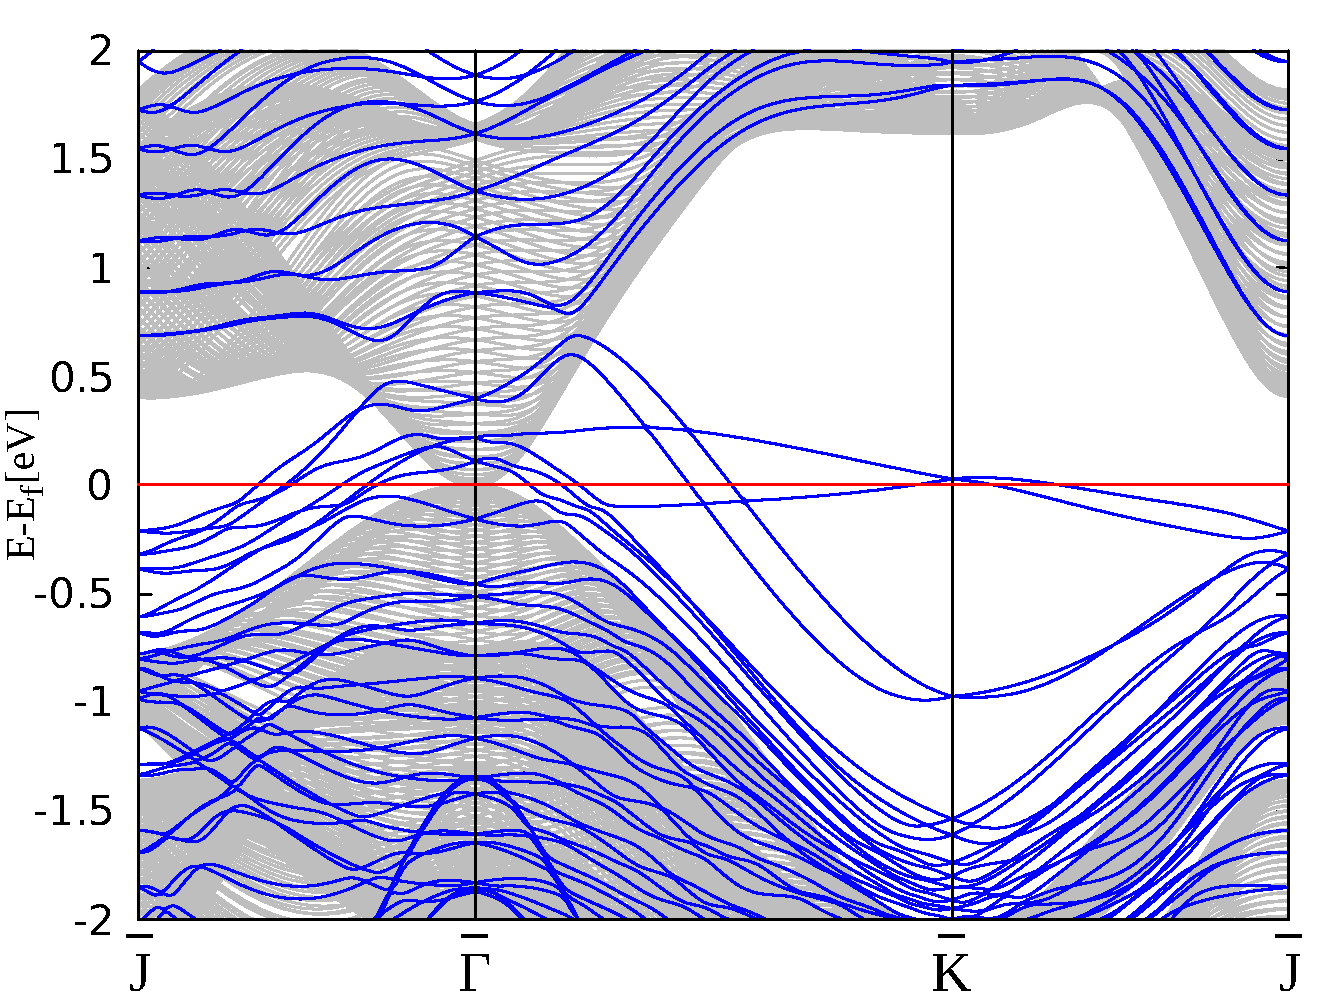
\includegraphics[width=\linewidth]{Hg_termination/bulk+17_layers_no_dos_-2_2.pdf}
			\caption{17 layers with hydrogens on the bottom passivating one of the Hg surface terminations}
		\end{subfigure}
		\caption{PBBS and surface band structure for symmetric Hg termination on both surfaces of the slab} 
		\label{bulk+surface_odd_layers_Hg}
	\end{figure}